\documentclass[10pt,fleqn]{article} % Default font size and left-justified equations
\usepackage[%
    pdftitle={SLCI : Systèmes du second ordre},
    pdfauthor={Xavier Pessoles}]{hyperref}

%%%%%%%%%%%%%%%%%%%%%%%%%%%%%%%%%%%%%%%%%
% Original author:
% Mathias Legrand (legrand.mathias@gmail.com) with modifications by:
% Vel (vel@latextemplates.com)
% License:
% CC BY-NC-SA 3.0 (http://creativecommons.org/licenses/by-nc-sa/3.0/)
%%%%%%%%%%%%%%%%%%%%%%%%%%%%%%%%%%%%%%%%%

%----------------------------------------------------------------------------------------
%	VARIOUS REQUIRED PACKAGES AND CONFIGURATIONS
%----------------------------------------------------------------------------------------

\usepackage[top=2.5cm,bottom=2cm,left=2cm,right=2cm,headsep=40pt,a4paper]{geometry} % Page margins

\usepackage{graphicx} % Required for including pictures
\graphicspath{{images/}} % Specifies the directory where pictures are stored

\usepackage{lipsum} % Inserts dummy text

\usepackage{tikz} % Required for drawing custom shapes

\usepackage[french]{babel} % English language/hyphenation
\frenchbsetup{StandardLists=true} % Pour éviter la collision babel enumitem pour les listes

\usepackage{enumitem} % Customize lists
\setlist{nolistsep} % Reduce spacing between bullet points and numbered lists

\usepackage{booktabs} % Required for nicer horizontal rules in tables

\usepackage{xcolor} % Required for specifying colors by name
%\definecolor{ocre}{RGB}{243,102,25} % Define the orange color used for highlighting throughout the book
 \definecolor{ocre}{RGB}{49,133,156} % Couleur ''bleue''
\definecolor{violetf}{RGB}{112,48,160} % Couleur ''violet''
\usepackage{enumitem}
\usepackage{pifont} % Pour les dinglist
\usepackage{multicol}
\usepackage{array} % Centrage vertical dans les tableaux

%----------------------------------------------------------------------------------------
%	FONTS
%----------------------------------------------------------------------------------------

\usepackage{avant} % Use the Avantgarde font for headings
%\usepackage{times} % Use the Times font for headings
%\usepackage{mathptmx} % Use the Adobe Times Roman as the default text font together with math symbols from the Sym­bol, Chancery and Com­puter Modern fonts
\usepackage[adobe-utopia]{mathdesign}
\usepackage{microtype} % Slightly tweak font spacing for aesthetics
\usepackage[utf8]{inputenc} % Required for including letters with accents
\usepackage[T1]{fontenc} % Use 8-bit encoding that has 256 glyphs

%----------------------------------------------------------------------------------------
%	BIBLIOGRAPHY AND INDEX
%----------------------------------------------------------------------------------------

\usepackage[style=alphabetic,citestyle=numeric,sorting=nyt,sortcites=true,autopunct=true,babel=hyphen,hyperref=true,abbreviate=false,backref=true,backend=biber]{biblatex}
\addbibresource{bibliography.bib} % BibTeX bibliography file
\defbibheading{bibempty}{}

\usepackage{calc} % For simpler calculation - used for spacing the index letter headings correctly
\usepackage{makeidx} % Required to make an index
\makeindex % Tells LaTeX to create the files required for indexing

%----------------------------------------------------------------------------------------
%	MAIN TABLE OF CONTENTS
%----------------------------------------------------------------------------------------

\usepackage{titletoc} % Required for manipulating the table of contents

\setcounter{tocdepth}{2}     % Dans la table des matieres
\setcounter{secnumdepth}{2}

\contentsmargin{0cm} % Removes the default margin

% Part text styling
\titlecontents{part}[0cm]
{\addvspace{20pt}\centering\large\bfseries}
{}
{}
{}

% Chapter text styling
\titlecontents{chapter}[1.25cm] % Indentation
{\addvspace{12pt}\large\sffamily\bfseries} % Spacing and font options for chapters
{\color{ocre!60}\contentslabel[\Large\thecontentslabel]{1.25cm}\color{ocre}} % Chapter number
{\color{ocre}}  
{\color{ocre!60}\normalsize\;\titlerule*[.5pc]{.}\;\thecontentspage} % Page number

% Section text styling
\titlecontents{section}[1.25cm] % Indentation
{\addvspace{3pt}\sffamily\bfseries} % Spacing and font options for sections
{\color{ocre!60}\contentslabel[\thecontentslabel]{1.25cm} \color{ocre}} % Section number
{\color{ocre}}
{\hfill\color{ocre!60}\thecontentspage} % Page number
[]

% Subsection text styling
\titlecontents{subsection}[1.25cm] % Indentation
{\addvspace{1pt}\sffamily\small} % Spacing and font options for subsections
{\contentslabel[\thecontentslabel]{1.25cm}} % Subsection number
{}
{\ \titlerule*[.5pc]{.}\;\thecontentspage} % Page number
[]


% Subsection text styling
\titlecontents{subsubsection}[1.25cm] % Indentation
{\addvspace{1pt}\sffamily\small} % Spacing and font options for subsections
{\contentslabel[\thecontentslabel]{1.25cm}} % Subsection number
{}
{\ \titlerule*[.5pc]{.}\;\thecontentspage} % Page number
[]

% List of figures
\titlecontents{figure}[0em]
{\addvspace{-5pt}\sffamily}
{\thecontentslabel\hspace*{1em}}
{}
{\ \titlerule*[.5pc]{.}\;\thecontentspage}
[]

% List of tables
\titlecontents{table}[0em]
{\addvspace{-5pt}\sffamily}
{\thecontentslabel\hspace*{1em}}
{}
{\ \titlerule*[.5pc]{.}\;\thecontentspage}
[]

%----------------------------------------------------------------------------------------
%	MINI TABLE OF CONTENTS IN PART HEADS
%----------------------------------------------------------------------------------------

% Chapter text styling
\titlecontents{lchapter}[0em] % Indenting
{\addvspace{15pt}\large\sffamily\bfseries} % Spacing and font options for chapters
{\color{ocre}\contentslabel[\Large\thecontentslabel]{1.25cm}\color{ocre}} % Chapter number
{}  
{\color{ocre}\normalsize\sffamily\bfseries\;\titlerule*[.5pc]{.}\;\thecontentspage} % Page number

% Section text styling
\titlecontents{lsection}[0em] % Indenting
{\sffamily\small} % Spacing and font options for sections
{\contentslabel[\thecontentslabel]{1.25cm}} % Section number
{}
{}

% Subsection text styling
\titlecontents{lsubsection}[.5em] % Indentation
{\normalfont\footnotesize\sffamily} % Font settings
{}
{}
{}

%----------------------------------------------------------------------------------------
%	PAGE HEADERS
%----------------------------------------------------------------------------------------

\usepackage{fancyhdr} % Required for header and footer configuration



\pagestyle{fancy}
 \renewcommand{\headrulewidth}{0pt}
 \fancyhead{}
 \fancyhead[L]{%
 \noindent\begin{minipage}[c]{2.6cm}%
 
\includegraphics[width=2cm]{png/logo_lycee.png}%
 \end{minipage}}

\fancyhead[C]{\rule{8cm}{.5pt}}

 \fancyhead[R]{%
 \noindent\begin{minipage}[c]{3cm}
 \begin{flushright}
 \footnotesize{\textit{\textsf{\xxtete}}}%
 \end{flushright}
 \end{minipage}
}


\fancyfoot[C]{\rule{12cm}{.5pt}}
\renewcommand{\footrulewidth}{0.2pt}
\fancyfoot[C]{\footnotesize{\bfseries \thepage}}
\fancyfoot[L]{ 
\begin{minipage}[c]{.4\linewidth}
\noindent\footnotesize{{\xxauteur}}
\end{minipage}}


\fancyfoot[R]{\footnotesize{\xxpied}
\ifthenelse{\isodd{\value{page}}}{
\begin{tikzpicture}[overlay]
\node[shape=rectangle, 
      rounded corners = .25 cm,
	  draw= ocre,
	  line width=2pt, 
	  fill = ocre!10,
	  minimum width  = 2.5cm,
	  minimum height = 3cm,] at (\xxposongletx,\xxposonglety) {};
\node at (\xxposonglettext,\xxposonglety) {\rotatebox{90}{\textbf{\large\color{ocre}{\xxonglet}}}};
%{};
\end{tikzpicture}}{}
}
%
%
%
% Removes the header from odd empty pages at the end of chapters
\makeatletter
\renewcommand{\cleardoublepage}{
\clearpage\ifodd\c@page\else
\hbox{}
\vspace*{\fill}
\thispagestyle{empty}
\newpage
\fi}

\fancypagestyle{plain}{%
\fancyhf{} % vide l’en-tête et le pied~de~page.
%\fancyfoot[C]{\bfseries \thepage} % numéro de la page en cours en gras
% et centré en pied~de~page.
\fancyfoot[R]{\footnotesize{\xxpied}}
\fancyfoot[C]{\rule{12cm}{.5pt}}
\renewcommand{\footrulewidth}{0.2pt}
\fancyfoot[C]{\footnotesize{\bfseries \thepage}}
\fancyfoot[L]{ 
\begin{minipage}[c]{.4\linewidth}
\noindent\footnotesize{{\xxauteur}}
\end{minipage}}}



%----------------------------------------------------------------------------------------
%	THEOREM STYLES
%----------------------------------------------------------------------------------------

% Conflit avec la police adobe
%\usepackage{amsmath,amsfonts,amssymb,amsthm} % For math equations, theorems, symbols, etc
\usepackage{amsmath,amsthm}

\newcommand{\intoo}[2]{\mathopen{]}#1\,;#2\mathclose{[}}
\newcommand{\ud}{\mathop{\mathrm{{}d}}\mathopen{}}
\newcommand{\intff}[2]{\mathopen{[}#1\,;#2\mathclose{]}}
%\newtheorem{notation}{Notation}[chapter]
\newtheorem{notation}{Notation}[section]

% Boxed/framed environments
\newtheoremstyle{ocrenumbox}% % Theorem style name
{0pt}% Space above
{0pt}% Space below
{\normalfont}% % Body font
{}% Indent amount
{\small\bf\sffamily\color{ocre}}% % Theorem head font
{\;}% Punctuation after theorem head
{0.25em}% Space after theorem head
{\small\sffamily\color{ocre}\thmname{#1}\nobreakspace\thmnumber%{\@ifnotempty{#1}{}\@upn{#2}}% Theorem text (e.g. Theorem 2.1)
\thmnote{\nobreakspace\the\thm@notefont\sffamily\bfseries\color{black}---\nobreakspace#3.}} % Optional theorem note
\renewcommand{\qedsymbol}{$\blacksquare$}% Optional qed square


% Boite pour les corriges
\newtheoremstyle{correctionbox}% % Theorem style name
{0pt}% Space above
{0pt}% Space below
{\normalfont}% % Body font
{}% Indent amount
{\small\bf\sffamily\color{violet}}% % Theorem head font
{\;}% Punctuation after theorem head
{0.25em}% Space after theorem head
{\small\sffamily\color{ocre}\thmname{#1}\nobreakspace\thmnumber%{\@ifnotempty{#1}{}\@upn{#2}}% Theorem text (e.g. Theorem 2.1)
\thmnote{\nobreakspace\the\thm@notefont\sffamily\bfseries\color{black}---\nobreakspace#3.}} % Optional theorem note
\renewcommand{\qedsymbol}{$\blacksquare$}% Optional qed square



\newtheoremstyle{blacknumex}% Theorem style name
{5pt}% Space above
{5pt}% Space below
{\normalfont}% Body font
{} % Indent amount
{\small\bf\sffamily}% Theorem head font
{\;}% Punctuation after theorem head
{0.25em}% Space after theorem head
{\small\sffamily{\tiny\ensuremath{\blacksquare}}\nobreakspace\thmname{#1}\nobreakspace\thmnumber%{\@ifnotempty{#1}{}\@upn{#2}}% Theorem text (e.g. Theorem 2.1)
\thmnote{\nobreakspace\the\thm@notefont\sffamily\bfseries---\nobreakspace#3.}}% Optional theorem note

\newtheoremstyle{blacknumbox} % Theorem style name
{0pt}% Space above
{0pt}% Space below
{\normalfont}% Body font
{}% Indent amount
{\small\bf\sffamily}% Theorem head font
{\;}% Punctuation after theorem head
{0.25em}% Space after theorem head
{\small\sffamily\thmname{#1}\nobreakspace 
\thmnote{\nobreakspace\the\thm@notefont\sffamily\bfseries---\nobreakspace#3.}}% Optional theorem note

% Non-boxed/non-framed environments
\newtheoremstyle{ocrenum}% % Theorem style name
{5pt}% Space above
{5pt}% Space below
{\normalfont}% % Body font
{}% Indent amount
{\small\bf\sffamily\color{ocre}}% % Theorem head font
{\;}% Punctuation after theorem head
{0.25em}% Space after theorem head
{\small\sffamily\color{ocre}\thmname{#1}\nobreakspace%\thmnumber{\@ifnotempty{#1}{}\@upn{#2}}% Theorem text (e.g. Theorem 2.1)
\thmnote{\nobreakspace\the\thm@notefont\sffamily\bfseries\color{black}---\nobreakspace#3.}} % Optional theorem note
\renewcommand{\qedsymbol}{$\blacksquare$}% Optional qed square
\makeatother

% Environnement pour les titres de parties
\newtheoremstyle{partiebox} 
{0pt}% Space above
{0pt}% Space below
{\normalfont}% Body font
{}% Indent amount
{\small\bf\sffamily}% Theorem head font
{\;}% Punctuation after theorem head
{0.25em}% Space after theorem head




% Defines the theorem text style for each type of theorem to one of the three styles above
\newcounter{dummy} 
\numberwithin{dummy}{section}
\theoremstyle{ocrenumbox}
%\newtheorem{theoremeT}[dummy]{Théorème}
\newtheorem{theoremeT}[dummy]{Théorème}
\newtheorem{resultatT}[dummy]{Résultat}
\newtheorem{savoirT}[dummy]{Savoir}
\newtheorem{methodeT}[dummy]{Méthode}
\newtheorem{objectifT}[dummy]{Objectif}
%\newtheorem{problem}{Problem}[chapter]
\newtheorem{problem}{Problem}[section]
%\newtheorem{exerciseT}{Exercise}[chapter]
\newtheorem{exerciseT}{Exercice}[section]

\theoremstyle{blacknumex}
%\newtheorem{exampleT}{Example}[chapter]
\newtheorem{exempleT}{Exemple}[section]
\newtheorem{termT}{Terminal\\}[section]
\newtheorem{pyT}{Python\\}[section]
\newtheorem{sciT}{Scilab\\}[section]
\newtheorem{pseudoT}{Pseudo Code\\}[section]
\newtheorem{sqlT}{SQL\\}[section]

\theoremstyle{blacknumbox}
%\newtheorem{vocabulary}{Vocabulary}[chapter]
\newtheorem{vocabulary}{Vocabulaire}[section]
%\newtheorem{definitionT}{Definition}[section]
\newtheorem{definitionT}{Définition}[section]
\newtheorem{rappelT}{Rappel}[section]
\newtheorem{demoT}{Démonstration}[section]
\newtheorem{corollaryT}[dummy]{Corollaire}
\newtheorem{hypoT}{Hypothèse(s)}

\theoremstyle{ocrenum}
\newtheorem{proposition}[dummy]{Proposition}

\theoremstyle{partiebox}
\newtheorem{titrepartieT}[]{}
\newtheorem{titrechapitreT}[]{}

\theoremstyle{correctionbox}
\newtheorem{correctionT}[dummy]{\color{violet}{Correction}}

%----------------------------------------------------------------------------------------
%	DEFINITION OF COLORED BOXES
%----------------------------------------------------------------------------------------

\RequirePackage[framemethod=tikz]{mdframed} % Required for creating the theorem, definition, exercise and corollary boxes

% Theorem box
\newmdenv[skipabove=7pt,
skipbelow=7pt,
backgroundcolor=ocre!10,
linecolor=ocre,
innerleftmargin=5pt,
innerrightmargin=5pt,
innertopmargin=5pt,
leftmargin=0cm,
rightmargin=0cm,
innerbottommargin=5pt]{tBox}


% Correction
\newmdenv[skipabove=7pt,
skipbelow=7pt,
backgroundcolor=violet!10,
linecolor=violet,
innerleftmargin=5pt,
innerrightmargin=5pt,
innertopmargin=5pt,
leftmargin=0cm,
rightmargin=0cm,
innerbottommargin=5pt]{coBox}


% Exercise box	  
\newmdenv[skipabove=7pt,
skipbelow=7pt,
rightline=false,
leftline=true,
topline=false,
bottomline=false,
backgroundcolor=ocre!10,
linecolor=ocre,
innerleftmargin=5pt,
innerrightmargin=5pt,
innertopmargin=5pt,
innerbottommargin=5pt,
leftmargin=0cm,
rightmargin=0cm,
linewidth=4pt]{eBox}	

% Definition box
\newmdenv[skipabove=7pt,
skipbelow=7pt,
rightline=false,
leftline=true,
topline=false,
bottomline=false,
backgroundcolor=ocre!10,
linecolor=ocre,
innerleftmargin=5pt,
innerrightmargin=5pt,
innertopmargin=0pt,
leftmargin=0cm,
rightmargin=0cm,
linewidth=4pt,
innerbottommargin=0pt]{dBox}	

% Demonstration box
\newmdenv[skipabove=7pt,
skipbelow=7pt,
rightline=false,
leftline=true,
topline=false,
bottomline=false,
%backgroundcolor=ocre!10,
linecolor=ocre,
innerleftmargin=5pt,
innerrightmargin=5pt,
innertopmargin=0pt,
leftmargin=0cm,
rightmargin=0cm,
linewidth=4pt,
innerbottommargin=0pt]{demoBox}	

% Corollary box
\newmdenv[skipabove=7pt,
skipbelow=7pt,
rightline=false,
leftline=true,
topline=false,
bottomline=false,
linecolor=gray,
backgroundcolor=black!5,
innerleftmargin=5pt,
innerrightmargin=5pt,
innertopmargin=5pt,
leftmargin=0cm,
rightmargin=0cm,
linewidth=4pt,
innerbottommargin=5pt]{cBox}


% Hypothèses
\newmdenv[skipabove=7pt,
skipbelow=7pt,
rightline=false,
leftline=true,
topline=false,
bottomline=false,
linecolor=gray,
backgroundcolor=black!5,
innerleftmargin=5pt,
innerrightmargin=5pt,
innertopmargin=5pt,
leftmargin=0cm,
rightmargin=0cm,
linewidth=4pt,
innerbottommargin=5pt]{hyBox}


% Boite pour le titre de la partie (pBox)
\newmdenv[skipabove=7pt,
skipbelow=7pt,
rightline=true,
leftline=false,
topline=false,
bottomline=false,
linecolor=ocre,
backgroundcolor=none,
innerleftmargin=5pt,
innerrightmargin=5pt,
innertopmargin=5pt,
leftmargin=0cm,
rightmargin=0cm,
linewidth=4pt,
innerbottommargin=5pt]{pBox}

% Boite pour le titre du chapitre (chBox)
\newmdenv[skipabove=7pt,
skipbelow=7pt,
rightline=false,
leftline=true,
topline=false,
bottomline=false,
linecolor=ocre,
%backgroundcolor=black!5,
innerleftmargin=5pt,
innerrightmargin=5pt,
innertopmargin=5pt,
leftmargin=0cm,
rightmargin=0cm,
linewidth=4pt,
innerbottommargin=5pt]{chBox}


% Boite pour les exemples
\newmdenv[skipabove=7pt,
skipbelow=7pt,
rightline=false,
leftline=true,
topline=false,
bottomline=false,
linecolor=gray,
backgroundcolor=white,
innerleftmargin=5pt,
innerrightmargin=5pt,
innertopmargin=5pt,
leftmargin=0cm,
rightmargin=0cm,
linewidth=4pt,
innerbottommargin=5pt]{exBox}

% Boite pour le terminal
\newmdenv[skipabove=7pt,
skipbelow=7pt,
rightline=false,
leftline=true,
topline=false,
bottomline=false,
linecolor=gray,
backgroundcolor=white,
innerleftmargin=5pt,
innerrightmargin=5pt,
innertopmargin=5pt,
leftmargin=0cm,
rightmargin=0cm,
linewidth=4pt,
innerbottommargin=5pt]{termBox}


% Boite pour Python
\newmdenv[skipabove=7pt,
skipbelow=7pt,
rightline=false,
leftline=true,
topline=false,
bottomline=false,
linecolor=gray,
backgroundcolor=white,
innerleftmargin=5pt,
innerrightmargin=5pt,
innertopmargin=0pt,
leftmargin=0cm,
rightmargin=0cm,
linewidth=4pt,
innerbottommargin=5pt]{pyBox}

% Boite pour scilab
\newmdenv[skipabove=7pt,
skipbelow=7pt,
rightline=false,
leftline=true,
topline=false,
bottomline=false,
linecolor=gray,
backgroundcolor=white,
innerleftmargin=5pt,
innerrightmargin=5pt,
innertopmargin=5pt,
leftmargin=0cm,
rightmargin=0cm,
linewidth=4pt,
innerbottommargin=5pt]{sciBox}


% Boite pour pseudo
\newmdenv[skipabove=7pt,
skipbelow=7pt,
rightline=false,
leftline=true,
topline=false,
bottomline=false,
linecolor=gray,
backgroundcolor=white,
innerleftmargin=5pt,
innerrightmargin=5pt,
innertopmargin=5pt,
leftmargin=0cm,
rightmargin=0cm,
linewidth=4pt,
innerbottommargin=5pt]{pseudoBox}

% Boite pour pseudo
\newmdenv[skipabove=7pt,
skipbelow=7pt,
rightline=false,
leftline=true,
topline=false,
bottomline=false,
linecolor=gray,
backgroundcolor=white,
innerleftmargin=5pt,
innerrightmargin=5pt,
innertopmargin=5pt,
leftmargin=0cm,
rightmargin=0cm,
linewidth=4pt,
innerbottommargin=5pt]{sqlBox}


% Creates an environment for each type of theorem and assigns it a theorem text style from the "Theorem Styles" section above and a colored box from above
\newenvironment{theorem}{\begin{tBox}\begin{theoremeT}}{\end{theoremeT}\end{tBox}}
\newenvironment{resultat}{\begin{tBox}\begin{resultatT}}{\end{resultatT}\end{tBox}}
\newenvironment{methode}{\begin{tBox}\begin{methodeT}}{\end{methodeT}\end{tBox}}
\newenvironment{savoir}{\begin{tBox}\begin{savoirT}}{\end{savoirT}\end{tBox}}
\newenvironment{obj}{\begin{tBox}\begin{objectifT}}{\end{objectifT}\end{tBox}}
\newenvironment{corrige}{\begin{coBox}\begin{correctionT}}{\end{correctionT}\end{coBox}}
\newenvironment{exercise}{\begin{eBox}\begin{exerciseT}}{\hfill{\color{ocre}\tiny\ensuremath{\blacksquare}}\end{exerciseT}\end{eBox}}				  
\newenvironment{exercice}{\begin{eBox}\begin{exerciseT}}{\hfill{\color{ocre}\tiny\ensuremath{\blacksquare}}\end{exerciseT}\end{eBox}}				  

\newenvironment{definition}{\begin{dBox}\begin{definitionT}}{\end{definitionT}\end{dBox}}	
\newenvironment{rappel}{\begin{dBox}\begin{rappelT}}{\end{rappelT}\end{dBox}}	
\newenvironment{defi}{\begin{dBox}\begin{definitionT}}{\end{definitionT}\end{dBox}}	
\newenvironment{demo}{\begin{demoBox}\begin{demoT}}{\end{demoT}\end{demoBox}}	
%\newenvironment{exemple}{\begin{exempleT}}{\hfill{\tiny\ensuremath{\blacksquare}}\end{exempleT}}		
\newenvironment{corollary}{\begin{cBox}\begin{corollaryT}}{\end{corollaryT}\end{cBox}}
\newenvironment{hypo}{\begin{hyBox}\begin{hypoT}}{\end{hypoT}\end{hyBox}}	\newenvironment{exemple}{\begin{exBox}\begin{exempleT}}{\hfill{\tiny\ensuremath{\blacksquare}}\end{exempleT}\end{exBox}}	
\newenvironment{titrepartie}{\begin{pBox}\begin{titrepartieT}}{\end{titrepartieT}\end{pBox}}	
\newenvironment{titrechapitre}{\begin{chBox}\begin{titrechapitreT}}{\end{titrechapitreT}\end{chBox}}	

\newenvironment{term}{ \begin{termBox}\begin{termT}}{\end{termT}\end{termBox}}
\newenvironment{py}{ \begin{pyBox}\begin{pyT}}{\end{pyT}\end{pyBox}}
\newenvironment{sci}{ \begin{sciBox}\begin{sciT}}{\end{sciT}\end{sciBox}}
\newenvironment{pseudo}{ \begin{pseudoBox}\begin{pseudoT}}{\end{pseudoT}\end{pseudoBox}}
\newenvironment{envsql}{ \begin{sqlBox}\begin{sqlT}}{\end{sqlT}\end{sqlBox}}


%----------------------------------------------------------------------------------------
%	REMARK ENVIRONMENT
%----------------------------------------------------------------------------------------

\newenvironment{remark}{\par\vspace{10pt}\small % Vertical white space above the remark and smaller font size
\begin{list}{}{
\leftmargin=35pt % Indentation on the left
\rightmargin=25pt}\item\ignorespaces % Indentation on the right
\makebox[-2.5pt]{\begin{tikzpicture}[overlay]
\node[draw=ocre!60,line width=1pt,circle,fill=ocre!25,font=\sffamily\bfseries,inner sep=2pt,outer sep=0pt] at (-15pt,0pt){\textcolor{ocre}{R}};\end{tikzpicture}} % Orange R in a circle
\advance\baselineskip -1pt}{\end{list}\vskip5pt} % Tighter line spacing and white space after remark

\newenvironment{rem}{\par\vspace{10pt}\small % Vertical white space above the remark and smaller font size
\begin{list}{}{
\leftmargin=35pt % Indentation on the left
\rightmargin=25pt}\item\ignorespaces % Indentation on the right
\makebox[-2.5pt]{\begin{tikzpicture}[overlay]
\node[draw=ocre!60,line width=1pt,circle,fill=ocre!25,font=\sffamily\bfseries,inner sep=2pt,outer sep=0pt] at (-15pt,0pt){\textcolor{ocre}{R}};\end{tikzpicture}} % Orange R in a circle
\advance\baselineskip -1pt}{\end{list}\vskip5pt} % Tighter line spacing and white space after remark


\newenvironment{warn}{\par\vspace{10pt}\small % Vertical white space above the remark and smaller font size
\begin{list}{}{
\leftmargin=35pt % Indentation on the left
\rightmargin=25pt}\item\ignorespaces % Indentation on the right
\makebox[-2.5pt]{\begin{tikzpicture}[overlay]
\node[draw=red!60,line width=1pt,circle,fill=red!25,font=\sffamily\bfseries,inner sep=2pt,outer sep=0pt] at (-15pt,0pt){\textcolor{black}{!}};\end{tikzpicture}} % Point d'exclamation dans un cercle
\advance\baselineskip -1pt}{\end{list}\vskip5pt} % Tighter line spacing and white space after remark


%----------------------------------------------------------------------------------------
%	SECTION NUMBERING IN THE MARGIN
%----------------------------------------------------------------------------------------
\setcounter{secnumdepth}{3}
\setcounter{tocdepth}{2}



\makeatletter
\renewcommand{\@seccntformat}[1]{\llap{\textcolor{ocre}{\csname the#1\endcsname}\hspace{1em}}}                    
\renewcommand{\section}{\@startsection{section}{1}{\z@}
{-4ex \@plus -1ex \@minus -.4ex}
{1ex \@plus.2ex }
{\normalfont\large\sffamily\bfseries}}
\renewcommand{\subsection}{\@startsection {subsection}{2}{\z@}
{-3ex \@plus -0.1ex \@minus -.4ex}
{0.5ex \@plus.2ex }
{\normalfont\sffamily\bfseries}}
\renewcommand{\subsubsection}{\@startsection {subsubsection}{3}{\z@}
{-2ex \@plus -0.1ex \@minus -.2ex}
{.2ex \@plus.2ex }
{\normalfont\small\sffamily\bfseries}}                        
\renewcommand\paragraph{\@startsection{paragraph}{4}{\z@}
{-2ex \@plus-.2ex \@minus .2ex}
{.1ex}
{\normalfont\small\sffamily\bfseries}}

%----------------------------------------------------------------------------------------
%	PART HEADINGS
%----------------------------------------------------------------------------------------


%----------------------------------------------------------------------------------------
%	CHAPTER HEADINGS
%----------------------------------------------------------------------------------------

% \newcommand{\thechapterimage}{}%
% \newcommand{\chapterimage}[1]{\renewcommand{\thechapterimage}{#1}}%
% \def\@makechapterhead#1{%
% {\parindent \z@ \raggedright \normalfont
% \ifnum \c@secnumdepth >\m@ne
% \if@mainmatter
% \begin{tikzpicture}[remember picture,overlay]
% \node at (current page.north west)
% {\begin{tikzpicture}[remember picture,overlay]
% \node[anchor=north west,inner sep=0pt] at (0,0) {\includegraphics[width=\paperwidth]{\thechapterimage}};
% \draw[anchor=west] (\Gm@lmargin,-9cm) node [line width=2pt,rounded corners=15pt,draw=ocre,fill=white,fill opacity=0.5,inner sep=15pt]{\strut\makebox[22cm]{}};
% \draw[anchor=west] (\Gm@lmargin+.3cm,-9cm) node {\huge\sffamily\bfseries\color{black}\thechapter. #1\strut};
% \end{tikzpicture}};
% \end{tikzpicture}
% \else
% \begin{tikzpicture}[remember picture,overlay]
% \node at (current page.north west)
% {\begin{tikzpicture}[remember picture,overlay]
% \node[anchor=north west,inner sep=0pt] at (0,0) {\includegraphics[width=\paperwidth]{\thechapterimage}};
% \draw[anchor=west] (\Gm@lmargin,-9cm) node [line width=2pt,rounded corners=15pt,draw=ocre,fill=white,fill opacity=0.5,inner sep=15pt]{\strut\makebox[22cm]{}};
% \draw[anchor=west] (\Gm@lmargin+.3cm,-9cm) node {\huge\sffamily\bfseries\color{black}#1\strut};
% \end{tikzpicture}};
% \end{tikzpicture}
% \fi\fi\par\vspace*{270\p@}}}

%-------------------------------------------

\def\@makeschapterhead#1{%
\begin{tikzpicture}[remember picture,overlay]
\node at (current page.north west)
{\begin{tikzpicture}[remember picture,overlay]
\node[anchor=north west,inner sep=0pt] at (0,0) {\includegraphics[width=\paperwidth]{\thechapterimage}};
\draw[anchor=west] (\Gm@lmargin,-9cm) node [line width=2pt,rounded corners=15pt,draw=ocre,fill=white,fill opacity=0.5,inner sep=15pt]{\strut\makebox[22cm]{}};
\draw[anchor=west] (\Gm@lmargin+.3cm,-9cm) node {\huge\sffamily\bfseries\color{black}#1\strut};
\end{tikzpicture}};
\end{tikzpicture}
\par\vspace*{270\p@}}
\makeatother

%----------------------------------------------------------------------------------------
%	HYPERLINKS IN THE DOCUMENTS
%----------------------------------------------------------------------------------------


\hypersetup{hidelinks,backref=true,pagebackref=true,hyperindex=true,colorlinks=false,breaklinks=true,urlcolor= ocre,bookmarks=true,bookmarksopen=false,pdftitle={Title},pdfauthor={Author}}
\usepackage{bookmark}
\bookmarksetup{
open,
numbered,
addtohook={%
\ifnum\bookmarkget{level}=0 % chapter
\bookmarksetup{bold}%
\fi
\ifnum\bookmarkget{level}=-1 % part
\bookmarksetup{color=ocre,bold}%
\fi
}
}

%----------------------------------------------------------------------------------------
%	
%----------------------------------------------------------------------------------------

\newcommand{\thechapterimage}{}%
\newcommand{\chapterimage}[1]{\renewcommand{\thechapterimage}{#1}}%
\def\@makechapterhead#1{%
{\parindent \z@ \raggedright \normalfont
\begin{tikzpicture}[remember picture,overlay]
\node at (current page.north west)
{\begin{tikzpicture}[remember picture,overlay]
\node[anchor=north west,inner sep=0pt] at (0,0) {\includegraphics[width=\paperwidth]{\thechapterimage}};
%\draw[anchor=west] (\Gm@lmargin,-9cm) node [line width=2pt,rounded corners=15pt,draw=ocre,fill=white,fill opacity=0.5,inner sep=15pt]{\strut\makebox[22cm]{}};
%\draw[anchor=west] (\Gm@lmargin+.3cm,-9cm) node {\huge\sffamily\bfseries\color{black}\thechapter. #1\strut};
\end{tikzpicture}};
\end{tikzpicture}
\par\vspace*{270\p@}
}}

 \newcounter{exo}


\makeatletter             
\renewcommand{\subparagraph}{\@startsection{exo}{5}{\z@}%
                                    {-2ex \@plus-.2ex \@minus .2ex}%
                                    {0ex}%               
{\normalfont\bfseries Question \hspace{.7cm} }}
\makeatother
\renewcommand{\thesubparagraph}{\arabic{subparagraph}} 
\makeatletter


%%%% Environnement pour inclure du code
\usepackage{textcomp}
\usepackage[french]{algorithm2e}
\usepackage{listings}
\lstloadlanguages{R}   % pour regler les pb d accent utf8 dans les codes
\lstset{language=R} % pour regler les pb d accent utf8 dans les codes
\renewcommand{\lstlistlistingname}{Listings}
\renewcommand{\lstlistingname}{Listing}

\SetKwBlock{Fonction}{Début Fonction}{Fin Fonction}
\SetKwComment{Comment}{start}{end}

\definecolor{Bleu}{rgb}{0.1,0.1,1.0}
\definecolor{Noir}{rgb}{0,0,0}
\definecolor{Grau}{rgb}{0.5,0.5,0.5}
\definecolor{DunkelGrau}{rgb}{0.15,0.15,0.15}
\definecolor{Hellbraun}{rgb}{0.5,0.25,0.0}
\definecolor{Magenta}{rgb}{1.0,0.0,1.0}
\definecolor{Gris}{gray}{0.5}
\definecolor{Vert}{rgb}{0,0.5,0}
\definecolor{SourceHintergrund}{rgb}{1,1.0,0.95}


\lstnewenvironment{python}[1][]{
\lstset{
%escapeinside={\%*}{*)},
inputencoding=utf8,   % pour regler les pb d accent utf8 dans les codes
extendedchars=true,   % pour regler les pb d accent utf8 dans les codes
language=python,
basicstyle=\ttfamily\footnotesize, 	
stringstyle=\color{red}, 
showstringspaces=false, 
alsoletter={1234567890},
otherkeywords={\ , \}, \{},
keywordstyle=\color{blue},
emph={access,and,break,class,continue,def,del,elif ,else,
except,exec,finally,for,from,global,if,import,in,i s,
lambda,not,or,pass,print,raise,return,try,while},
emphstyle=\color{black}\bfseries,
emph={[2]True, False, None, self},
emphstyle=[2]\color{black},
emph={[3]from, import, as},
emphstyle=[3]\color{blue},
upquote=true,
columns=flexible, % pour empecher d'avoir un espacement mono
morecomment=[s]{"""}{"""},
commentstyle=\color{Hellbraun}\slshape, 
%emph={[4]1, 2, 3, 4, 5, 6, 7, 8, 9, 0},
emphstyle=[4]\color{blue},
literate=*{:}{{\textcolor{blue}:}}{1}
{=}{{\textcolor{blue}=}}{1}
{-}{{\textcolor{blue}-}}{1}
{+}{{\textcolor{blue}+}}{1}
{*}{{\textcolor{blue}*}}{1}
{!}{{\textcolor{blue}!}}{1}
{(}{{\textcolor{blue}(}}{1}
{)}{{\textcolor{blue})}}{1}
{[}{{\textcolor{blue}[}}{1}
{]}{{\textcolor{blue}]}}{1}
{<}{{\textcolor{blue}<}}{1}
{>}{{\textcolor{blue}>}}{1}
{COMPLETER}{{\textcolor{red}COMPLETER}}{1},
literate=%
            {é}{{\'{e}}}1
            {è}{{\`{e}}}1
            {ê}{{\^{e}}}1
            {ë}{{\¨{e}}}1
            {û}{{\^{u}}}1
            {ù}{{\`{u}}}1
            {â}{{\^{a}}}1
            {à}{{\`{a}}}1
            {î}{{\^{i}}}1
            {ç}{{\c{c}}}1
            {Ç}{{\c{C}}}1
            {É}{{\'{E}}}1
            {Ê}{{\^{E}}}1
            {À}{{\`{A}}}1
            {Â}{{\^{A}}}1
            {Î}{{\^{I}}}1, % pour regler les pb d accent utf8 dans les codes
%framexleftmargin=1mm, framextopmargin=1mm, frame=shadowbox, rulesepcolor=\color{blue},#1
%backgroundcolor=\color{SourceHintergrund}, 
%framexleftmargin=1mm, framexrightmargin=1mm, framextopmargin=1mm, frame=single, framerule=1pt, rulecolor=\color{black},#1
}}{}



\lstnewenvironment{scilab}[1][]{
\lstset{
language=scilab,
basicstyle=\sffamily\footnotesize, 	
stringstyle=\color{red}, 
showstringspaces=false, 
alsoletter={1234567890},
otherkeywords={\ , \}, \{},
keywordstyle=\color{blue},
emph={access,and,break,class,continue,def,del,elif ,else,
except,exec,finally,for,from,global,if,import,in,i s,
lambda,not,or,pass,print,raise,return,try,while,Debut},
emphstyle=\color{black}\bfseries,
emph={[2]True, False, None, self},
emphstyle=[2]\color{black},
emph={[3]from, import, as},
emphstyle=[3]\color{blue},
upquote=true,
columns=flexible, % pour empecher d'avoir un espacement mono
morecomment=[s]{"""}{"""},
commentstyle=\color{Hellbraun}\slshape, 
%emph={[4]1, 2, 3, 4, 5, 6, 7, 8, 9, 0},
emphstyle=[4]\color{blue},
literate=*{:}{{\textcolor{blue}:}}{1}
{=}{{\textcolor{blue}=}}{1}
{-}{{\textcolor{blue}-}}{1}
{+}{{\textcolor{blue}+}}{1}
{*}{{\textcolor{blue}*}}{1}
{!}{{\textcolor{blue}!}}{1}
{(}{{\textcolor{blue}(}}{1}
{)}{{\textcolor{blue})}}{1}
{[}{{\textcolor{blue}[}}{1}
{]}{{\textcolor{blue}]}}{1}
{<}{{\textcolor{blue}<}}{1}
{>}{{\textcolor{blue}>}}{1},
%framexleftmargin=1mm, framextopmargin=1mm, frame=shadowbox, rulesepcolor=\color{blue},#1
%backgroundcolor=\color{SourceHintergrund}, 
%framexleftmargin=1mm, framexrightmargin=1mm, framextopmargin=1mm, frame=single, framerule=1pt, rulecolor=\color{black},#1
}}{}


\lstdefinestyle{stylepython}{%
escapeinside={\%*}{*)},
inputencoding=utf8,   % pour regler les pb d accent utf8 dans les codes
extendedchars=true,   % pour regler les pb d accent utf8 dans les codes
language=python,
basicstyle=\sffamily\footnotesize, 	
stringstyle=\color{red}, 
showstringspaces=false, 
alsoletter={1234567890},
otherkeywords={\ , \}, \{},
keywordstyle=\color{blue},
emph={access,and,break,class,continue,def,del,elif ,else,
except,exec,finally,for,from,global,if,import,in,i s,
lambda,not,or,pass,print,raise,return,try,while},
emphstyle=\color{black}\bfseries,
emph={[2]True, False, None, self},
emphstyle=[2]\color{green},
emph={[3]from, import, as},
emphstyle=[3]\color{blue},
upquote=true,
columns=flexible, % pour empecher d'avoir un espacement mono
morecomment=[s]{"""}{"""},
commentstyle=\color{Hellbraun}\slshape, 
%emph={[4]1, 2, 3, 4, 5, 6, 7, 8, 9, 0},
emphstyle=[4]\color{blue},
literate=*{:}{{\textcolor{blue}:}}{1}
{=}{{\textcolor{blue}=}}{1}
{-}{{\textcolor{blue}-}}{1}
{+}{{\textcolor{blue}+}}{1}
{*}{{\textcolor{blue}*}}{1}
{!}{{\textcolor{blue}!}}{1}
{(}{{\textcolor{blue}(}}{1}
{)}{{\textcolor{blue})}}{1}
{[}{{\textcolor{blue}[}}{1}
{]}{{\textcolor{blue}]}}{1}
{<}{{\textcolor{blue}<}}{1}
{>}{{\textcolor{blue}>}}{1}
{COMPLETER}{{\textcolor{red}COMPLETER}}{1},
literate=%
            {é}{{\'{e}}}1
            {è}{{\`{e}}}1
            {ê}{{\^{e}}}1
            {ë}{{\¨{e}}}1
            {û}{{\^{u}}}1
            {ù}{{\`{u}}}1
            {â}{{\^{a}}}1
            {à}{{\`{a}}}1
            {î}{{\^{i}}}1
            {ç}{{\c{c}}}1
            {Ç}{{\c{C}}}1
            {É}{{\'{E}}}1
            {Ê}{{\^{E}}}1
            {À}{{\`{A}}}1
            {Â}{{\^{A}}}1
            {Î}{{\^{I}}}1,
%numbers=left,                    % where to put the line-numbers; possible values are (none, left, right)
%numbersep=5pt,                   % how far the line-numbers are from the code
%numberstyle=\tiny\color{mygray}, % the style that is used for the line-numbers
}



\lstnewenvironment{termi}[1][]{
\lstset{
language=scilab,
basicstyle=\sffamily\footnotesize, 	
stringstyle=\color{red}, 
showstringspaces=false, 
alsoletter={1234567890},
otherkeywords={\ , \}, \{},
keywordstyle=\color{blue},
emph={access,and,break,class,continue,def,del,elif ,else,
except,exec,finally,for,from,global,if,import,in,i s,
lambda,not,or,pass,print,raise,return,try,while,Debut},
emphstyle=\color{black}\bfseries,
emph={[2]True, False, None, self},
emphstyle=[2]\color{green},
emph={[3]from, import, as},
emphstyle=[3]\color{blue},
upquote=true,
columns=flexible, % pour empecher d'avoir un espacement mono
morecomment=[s]{"""}{"""},
commentstyle=\color{Hellbraun}\slshape, 
%emph={[4]1, 2, 3, 4, 5, 6, 7, 8, 9, 0},
emphstyle=[4]\color{blue},
literate=*{:}{{\textcolor{blue}:}}{1}
{=}{{\textcolor{blue}=}}{1}
{-}{{\textcolor{blue}-}}{1}
{+}{{\textcolor{blue}+}}{1}
{*}{{\textcolor{blue}*}}{1}
{!}{{\textcolor{blue}!}}{1}
{(}{{\textcolor{blue}(}}{1}
{)}{{\textcolor{blue})}}{1}
{[}{{\textcolor{blue}[}}{1}
{]}{{\textcolor{blue}]}}{1}
{<}{{\textcolor{blue}<}}{1}
{>}{{\textcolor{blue}>}}{1},
%framexleftmargin=1mm, framextopmargin=1mm, frame=shadowbox, rulesepcolor=\color{blue},#1
%backgroundcolor=\color{SourceHintergrund}, 
%framexleftmargin=1mm, framexrightmargin=1mm, framextopmargin=1mm, frame=single, framerule=1pt, rulecolor=\color{black},#1
}}{}


\lstnewenvironment{sql}[1][]{
\lstset{
%escapeinside={\%*}{*)},
%inputencoding=utf8,   % pour regler les pb d accent utf8 dans les codes
%extendedchars=true,   % pour regler les pb d accent utf8 dans les codes
language=sql,
basicstyle=\sffamily\footnotesize, 	
stringstyle=\color{red}, 
showstringspaces=false, 
alsoletter={1234567890},
otherkeywords={\ , \}, \{},
keywordstyle=\color{blue},
emph={access,and,break,class,continue,def,del,elif ,else,
except,exec,finally,for,from,global,if,import,in,i s,
lambda,not,or,pass,print,raise,return,try,while},
emphstyle=\color{black}\bfseries,
emph={[2]True, False, None, self},
emphstyle=[2]\color{black},
emph={[3]from, import, as},
emphstyle=[3]\color{blue},
upquote=true,
columns=flexible, % pour empecher d'avoir un espacement mono
morecomment=[s]{"""}{"""},
commentstyle=\color{Hellbraun}\slshape, 
%emph={[4]1, 2, 3, 4, 5, 6, 7, 8, 9, 0},
emphstyle=[4]\color{blue},
literate=*{:}{{\textcolor{blue}:}}{1}
{=}{{\textcolor{blue}=}}{1}
{-}{{\textcolor{blue}-}}{1}
{+}{{\textcolor{blue}+}}{1}
{*}{{\textcolor{blue}*}}{1}
{!}{{\textcolor{blue}!}}{1}
{(}{{\textcolor{blue}(}}{1}
{)}{{\textcolor{blue})}}{1}
{[}{{\textcolor{blue}[}}{1}
{]}{{\textcolor{blue}]}}{1}
{<}{{\textcolor{blue}<}}{1}
{>}{{\textcolor{blue}>}}{1}
{COMPLETER}{{\textcolor{red}COMPLETER}}{1},
literate=%
            {é}{{\'{e}}}1
            {è}{{\`{e}}}1
            {ê}{{\^{e}}}1
            {ë}{{\¨{e}}}1
            {û}{{\^{u}}}1
            {ù}{{\`{u}}}1
            {â}{{\^{a}}}1
            {à}{{\`{a}}}1
            {î}{{\^{i}}}1
            {ç}{{\c{c}}}1
            {Ç}{{\c{C}}}1
            {É}{{\'{E}}}1
            {Ê}{{\^{E}}}1
            {À}{{\`{A}}}1
            {Â}{{\^{A}}}1
            {Î}{{\^{I}}}1, % pour regler les pb d accent utf8 dans les codes
%framexleftmargin=1mm, framextopmargin=1mm, frame=shadowbox, rulesepcolor=\color{blue},#1
%backgroundcolor=\color{SourceHintergrund}, 
%framexleftmargin=1mm, framexrightmargin=1mm, framextopmargin=1mm, frame=single, framerule=1pt, rulecolor=\color{black},#1
}}{}


% Définition des booleéns
\newif\iffiche
\newif\ifprof
\newif\iftd
\newif\ifcours

%%%%%%%%%%%%
% Définition des vecteurs 
%%%%%%%%%%%%
 \newcommand{\vect}[1]{\overrightarrow{#1}}
\newcommand{\axe}[2]{\left(#1,\vect{#2}\right)}

\newcommand{\rep}[1]{\mathcal{R}_{#1}}
\newcommand{\vx}[1]{\vect{x_{#1}}}
\newcommand{\vy}[1]{\vect{y_{#1}}}
\newcommand{\vz}[1]{\vect{z_{#1}}}

%%%%%%%%%%%%
% Définition des torseurs 
%%%%%%%%%%%%

 \newcommand{\torseur}[1]{%
\left\{{#1}\right\}
}

\newcommand{\torseurcin}[3]{%
\left\{\mathcal{#1} \left(#2/#3 \right) \right\}
}

\newcommand{\torseurstat}[3]{%
\left\{\mathcal{#1} \left(#2\rightarrow #3 \right) \right\}
}

 \newcommand{\torseurc}[8]{%
%\left\{#1 \right\}=
\left\{
{#1}
\right\}
 = 
\left\{%
\begin{array}{cc}%
{#2} & {#5}\\%
{#3} & {#6}\\%
{#4} & {#7}\\%
\end{array}%
\right\}_{#8}%
}

 \newcommand{\torseurcol}[7]{
\left\{%
\begin{array}{cc}%
{#1} & {#4}\\%
{#2} & {#5}\\%
{#3} & {#6}\\%
\end{array}%
\right\}_{#7}%
}

 \newcommand{\torseurl}[3]{%
%\left\{\mathcal{#1}\right\}_{#2}=%
\left\{%
\begin{array}{l}%
{#1} \\%
{#2} %
\end{array}%
\right\}_{#3}%
}

 \newcommand{\vectv}[3]{%
\vect{V\left( {#1} \in {#2}/{#3}\right)}
}


\newcommand{\vectf}[2]{%
\vect{R\left( {#1} \rightarrow {#2}\right)}
}

\newcommand{\vectm}[3]{%
\vect{\mathcal{M}\left( {#1}, {#2} \rightarrow {#3}\right)}
}


 \newcommand{\vectg}[3]{%
\vect{\Gamma \left( {#1} \in {#2}/{#3}\right)}
}

 \newcommand{\vecto}[2]{%
\vect{\Omega\left( {#1}/{#2}\right)}
}
% }$$\left\{\mathcal{#1} \right\}_{#2} =%
% \left\{%
% \begin{array}{c}%
%  #3 \\%
%  #4 %
% \end{array}%
% \right\}_{#5}}

\usepackage{multicol}
\fichetrue
%\fichefalse

%\proftrue
\proffalse

\tdtrue
%\tdfalse

\courstrue
\coursfalse

\def\discipline{Sciences \\Industrielles de \\ l'Ingénieur}
\def\xxtete{Sciences Industrielles de l'Ingénieur}

\def\classe{PTSI}
\def\xxnumpartie{Partie 2}
\def\xxpartie{Découverte des Systèmes Linéaires Continus et Invariants\\
Analyse, Modélisation, Résolution}


\def\xxnumchapitre{Chapitre 5}
\def\xxchapitre{\hspace{.12cm} Étude des systèmes fondamentaux du second ordre}

\def\xxtitreexo{}%Prothèse Active Transtibiale}
\def\xxsourceexo{}%\hspace{.2cm} D'après concours Mines-Ponts -- 2013.}


\def\xxposongletx{2}
\def\xxposonglettext{1.45}
\def\xxposonglety{20}
\def\xxonglet{Part. 2 -- Ch. 5}

\def\xxactivite{Applications}
\def\xxauteur{\textsl{Florestan Mathurin -- Alain Caignot}}

\def\xxcompetences{%
\textsl{%
\textbf{Savoirs et compétences :}
\begin{itemize}[label=\ding{112},font=\color{ocre}] 
\item Mod-C2.3 : Modèles canoniques du second ordre
\begin{itemize}[label=\ding{112},font=\color{ocre}] 
\item Mod-C2-S1 : Identifier le comportement d’un système pour l’assimiler à un modèle canonique, à partir d’une réponse temporelle 
\item Mod-C2-S2 : Établir un modèle de comportement à partir de relevés expérimentaux
\end{itemize}
\end{itemize}
}}


\def\xxfigures{
%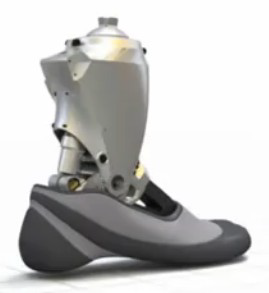
\includegraphics[width=.8\linewidth]{images/prot_01}
}%figues de la page de garde

\def\xxpied{%
Partie 3 -- Étude cinématique des systèmes  \\
Ch 5 : Cinématique du solide -- \xxactivite%
}


\setcounter{secnumdepth}{5}
%---------------------------------------------------------------------------


\begin{document}
%\chapterimage{images/Fond_Cin}
\pagestyle{empty}


%%%%%%%% PAGE DE GARDE COURS
\ifcours
\begin{tikzpicture}[remember picture,overlay]
\node at (current page.north west)
{\begin{tikzpicture}[remember picture,overlay]
\node[anchor=north west,inner sep=0pt] at (0,0) {\includegraphics[width=\paperwidth]{\thechapterimage}};
\draw[anchor=west] (-2cm,-8cm) node [line width=2pt,rounded corners=15pt,draw=ocre,fill=white,fill opacity=0.6,inner sep=40pt]{\strut\makebox[22cm]{}};
\draw[anchor=west] (1cm,-8cm) node {\huge\sffamily\bfseries\color{black} %
\begin{minipage}{1cm}
\rotatebox{90}{\LARGE\sffamily\textsc{\color{ocre}\textbf{\xxnumpartie}}}
\end{minipage} \hfill
\begin{minipage}[c]{14cm}
\begin{titrepartie}
\begin{flushright}
\renewcommand{\baselinestretch}{1.1} 
\Large\sffamily\textsc{\textbf{\xxpartie}}
\renewcommand{\baselinestretch}{1} 
\end{flushright}
\end{titrepartie}
\end{minipage} \hfill
\begin{minipage}[c]{3.5cm}
{\large\sffamily\textsc{\textbf{\color{ocre} \discipline}}}
\end{minipage} 
 };
\end{tikzpicture}};
\end{tikzpicture}


\begin{tikzpicture}[overlay]
\node[shape=rectangle, 
      rounded corners = .25 cm,
	  draw= ocre,
	  line width=2pt, 
	  fill = ocre!10,
	  minimum width  = 2.5cm,
	  minimum height = 3cm,] at (18cm,0) {};
\node at (17.7cm,0) {\rotatebox{90}{\textbf{\Large\color{ocre}{\classe}}}};
%{};
\end{tikzpicture}

\vspace{3.5cm}

\begin{tikzpicture}[remember picture,overlay]
\draw[anchor=west] (-2cm,-6cm) node {\huge\sffamily\bfseries\color{black} %
\begin{minipage}{2cm}
\begin{center}
\LARGE\sffamily\textsc{\color{ocre}\textbf{\xxactivite}}
\end{center}
\end{minipage} \hfill
\begin{minipage}[c]{15cm}
\begin{titrechapitre}
\renewcommand{\baselinestretch}{1.1} 
\Large\sffamily\textsc{\textbf{\xxnumchapitre}}

\Large\sffamily\textsc{\textbf{\xxchapitre}}
\vspace{.5cm}

\renewcommand{\baselinestretch}{1} 
\normalsize\normalfont
\xxcompetences
\end{titrechapitre}
\end{minipage}  };
\end{tikzpicture}
\vfill

\begin{flushright}
\begin{minipage}[c]{.3\linewidth}
\begin{center}
\xxfigures
\end{center}
\end{minipage}\hfill
\begin{minipage}[c]{.6\linewidth}
\startcontents
\printcontents{}{1}{}
\end{minipage}
\end{flushright}

\begin{tikzpicture}[remember picture,overlay]
\draw[anchor=west] (4.5cm,-.7cm) node {
\begin{minipage}[c]{.2\linewidth}
\begin{flushright}

\includegraphics[width=2cm]{png/logoCC}
\end{flushright}
\end{minipage}
\begin{minipage}[c]{.2\linewidth}
\textsl{\xxauteur} \\
\textsl{\classe}
\end{minipage}
 };
\end{tikzpicture}
\newpage
\pagestyle{fancy}

\newpage
\pagestyle{fancy}

\else
\fi


%%%%%%%% PAGE DE GARDE TD
\iftd
%\begin{tikzpicture}[remember picture,overlay]
%\node at (current page.north west)
%{\begin{tikzpicture}[remember picture,overlay]
%\draw[anchor=west] (-2cm,-3.25cm) node [line width=2pt,rounded corners=15pt,draw=ocre,fill=white,fill opacity=0.6,inner sep=40pt]{\strut\makebox[22cm]{}};
%\draw[anchor=west] (1cm,-3.25cm) node {\huge\sffamily\bfseries\color{black} %
%\begin{minipage}{1cm}
%\rotatebox{90}{\LARGE\sffamily\textsc{\color{ocre}\textbf{\xxnumpartie}}}
%\end{minipage} \hfill
%\begin{minipage}[c]{13.5cm}
%\begin{titrepartie}
%\begin{flushright}
%\renewcommand{\baselinestretch}{1.1} 
%\Large\sffamily\textsc{\textbf{\xxpartie}}
%\renewcommand{\baselinestretch}{1} 
%\end{flushright}
%\end{titrepartie}
%\end{minipage} \hfill
%\begin{minipage}[c]{3.5cm}
%{\large\sffamily\textsc{\textbf{\color{ocre} \discipline}}}
%\end{minipage} 
% };
%\end{tikzpicture}};
%\end{tikzpicture}

%%%%%%%%%% PAGE DE GARDE TD %%%%%%%%%%%%%%%
%\begin{tikzpicture}[overlay]
%\node[shape=rectangle, 
%      rounded corners = .25 cm,
%	  draw= ocre,
%	  line width=2pt, 
%	  fill = ocre!10,
%	  minimum width  = 2.5cm,
%	  minimum height = 2.5cm,] at (18.5cm,0) {};
%\node at (17.7cm,0) {\rotatebox{90}{\textbf{\Large\color{ocre}{\classe}}}};
%%{};
%\end{tikzpicture}

% PARTIE ET CHAPITRE
%\begin{tikzpicture}[remember picture,overlay]
%\draw[anchor=west] (-1cm,-2.1cm) node {\large\sffamily\bfseries\color{black} %
%\begin{minipage}[c]{15cm}
%\begin{flushleft}
%\xxnumchapitre \\
%\xxchapitre
%\end{flushleft}
%\end{minipage}  };
%\end{tikzpicture}

% Bandeau titre exo
\begin{tikzpicture}[remember picture,overlay]
\draw[anchor=west] (-2cm,-6cm) node {\huge\sffamily\bfseries\color{black} %
\begin{minipage}{5cm}
\begin{center}
\LARGE\sffamily\color{ocre}\textbf{\textsc{\xxactivite}}

\begin{center}
\xxfigures
\end{center}

\end{center}
\end{minipage} \hfill
\begin{minipage}[c]{12cm}
\begin{titrechapitre}
\renewcommand{\baselinestretch}{1.1} 
\large\sffamily\textbf{\textsc{\xxtitreexo}}

\small\sffamily{\textbf{\textit{\color{black!70}\xxsourceexo}}}
\vspace{.5cm}

\renewcommand{\baselinestretch}{1} 
\normalsize\normalfont
\xxcompetences
\end{titrechapitre}
\end{minipage}  };
\end{tikzpicture}

\else
\fi


%%%%%%%% PAGE DE GARDE FICHE
\iffiche
\begin{tikzpicture}[remember picture,overlay]
\node at (current page.north west)
{\begin{tikzpicture}[remember picture,overlay]
\draw[anchor=west] (-2cm,-3.25cm) node [line width=2pt,rounded corners=15pt,draw=ocre,fill=white,fill opacity=0.6,inner sep=40pt]{\strut\makebox[22cm]{}};
\draw[anchor=west] (1cm,-3.25cm) node {\huge\sffamily\bfseries\color{black} %
\begin{minipage}{1cm}
\rotatebox{90}{\LARGE\sffamily\textsc{\color{ocre}\textbf{\xxnumpartie}}}
\end{minipage} \hfill
\begin{minipage}[c]{14cm}
\begin{titrepartie}
\begin{flushright}
\renewcommand{\baselinestretch}{1.1} 
\large\sffamily\textsc{\textbf{\xxpartie} \\} 

\vspace{.2cm}

\normalsize\sffamily\textsc{\textbf{\xxnumchapitre -- \xxchapitre}}
\renewcommand{\baselinestretch}{1} 
\end{flushright}
\end{titrepartie}
\end{minipage} \hfill
\begin{minipage}[c]{3.5cm}
{\large\sffamily\textsc{\textbf{\color{ocre} \discipline}}}
\end{minipage} 
 };
\end{tikzpicture}};
\end{tikzpicture}


\begin{tikzpicture}[overlay]
\node[shape=rectangle, 
      rounded corners = .25 cm,
	  draw= ocre,
	  line width=2pt, 
	  fill = ocre!10,
	  minimum width  = 2.5cm,
	  minimum height = 2.5cm,] at (18.5cm,0.5cm) {};
%	  minimum height = 2.5cm,] at (18.5cm,0cm) {};
\node at (17.7cm,0.5) {\rotatebox{90}{\textsf{\textbf{\large\color{ocre}{\classe}}}}};
%{};
\end{tikzpicture}



\else
\fi



\vspace{8cm}
\pagestyle{fancy}
\thispagestyle{plain}


\def\columnseprulecolor{\color{ocre}}
\setlength{\columnseprule}{0.4pt} 
\begin{multicols}{2}


\section*{Correcteur de phare}
\begin{flushright}
\textit{D'après ressources de Florestan Mathurin -- concours CCP PSI 2003.}
\end{flushright}


\subsection*{Présentation du système}

L‘assiette d‘un véhicule se modifie avec sa charge, le profil de la route ou les
conditions de conduite (phase de freinage ou d‘accélération). Cette modification
entraîne une variation d‘inclinaison de l‘axe du faisceau lumineux produit par
les phares du véhicule. Ceux ci peuvent alors éblouir d‘autres conducteurs ou
mal éclairer la chaussée.


\begin{center}
 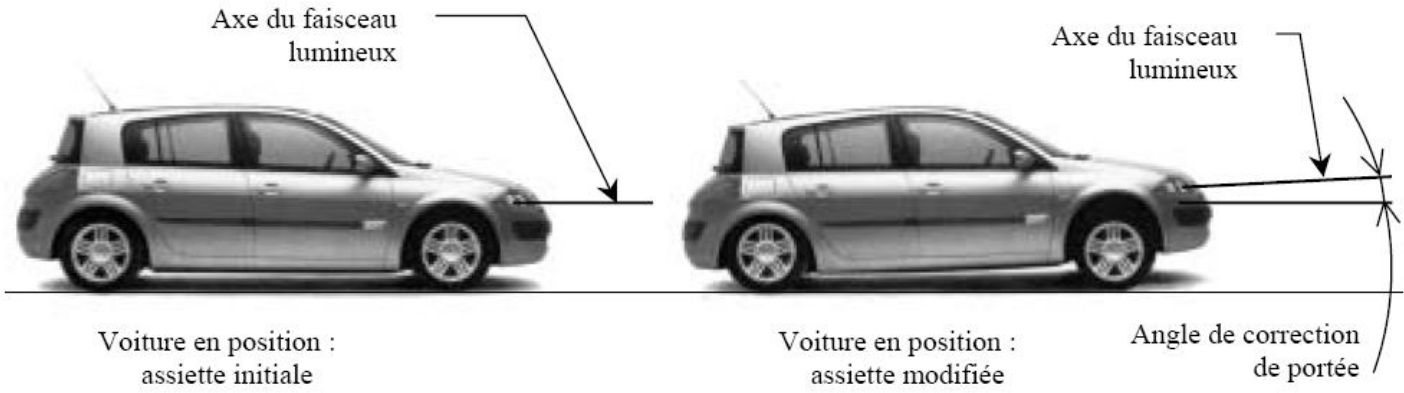
\includegraphics[width=.9\linewidth]{images/image1_1}
\end{center}
     
         Certaines voitures sont équipées de système de correction de portée. Ce
système fait appel à
des capteurs d‘assiette reliés aux essieux avant et arrière du véhicule. Les
données sont traitées
électroniquement par un calculateur et transmises aux actionneurs situés
derrière les projecteurs. La
position du projecteur est ajustée en maintenant un angle de faisceau optimal
évitant tout
éblouissement et fournissant le meilleur éclairage de la route.
Le système étudié est un correcteur de portée statique, qui corrige la portée
lorsque le véhicule est à
l‘arrêt et conserve cette correction lorsque le véhicule roule (le correcteur ne
tient compte que de la
variation d‘assiette due à la charge).

       Le but de l‘étude est d‘analyser le système et de montrer s‘il est
capable de corriger la portée
de manière dynamique, c‘est à dire en tenant compte des variations d‘assiette
dues au profil de la
route.

\subsubsection*{Éléments constitutifs du correcteur de portée}

\textbf{Capteurs d’assiette} : codeurs optiques permettant de mesurer le
débattement des suspensions.

\textbf{Système d’orientation : bloc d’orientation + moto-réducteur + système
vis écrou}

Le bloc d‘orientation supporte les différentes lampes du phare (codes,
clignotants...). Il peut pivoter
par rapport au support lié à la carrosserie autour d‘un axe horizontal (axe de
rotation indiqué sur la
figure ci-dessous). Le bloc est protégé par une vitre liée à la carrosserie. Ce
mouvement est motorisé
grâce au moto-réducteur + système vis écrou. Il existe aussi une possibilité de
réglage manuel en
sortie d‘usine ou en cas de défaillance du système électrique.

\begin{center}
 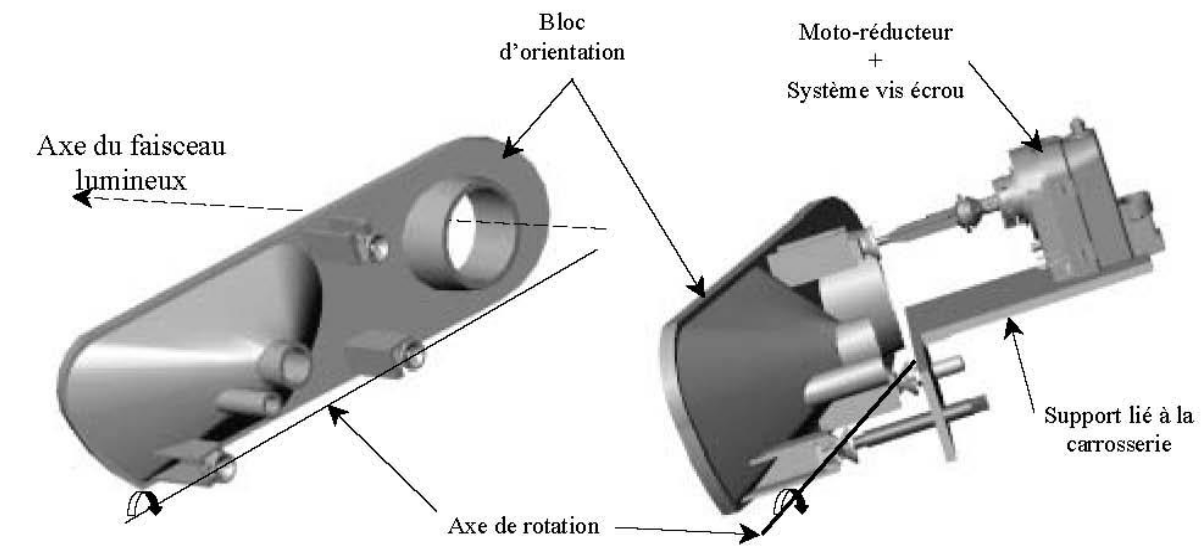
\includegraphics[width=.9\linewidth]{images/image1_2}
\end{center}

\subsubsection*{Diagrammes SADT niveau A-0, A0 et A3}
\begin{center}
 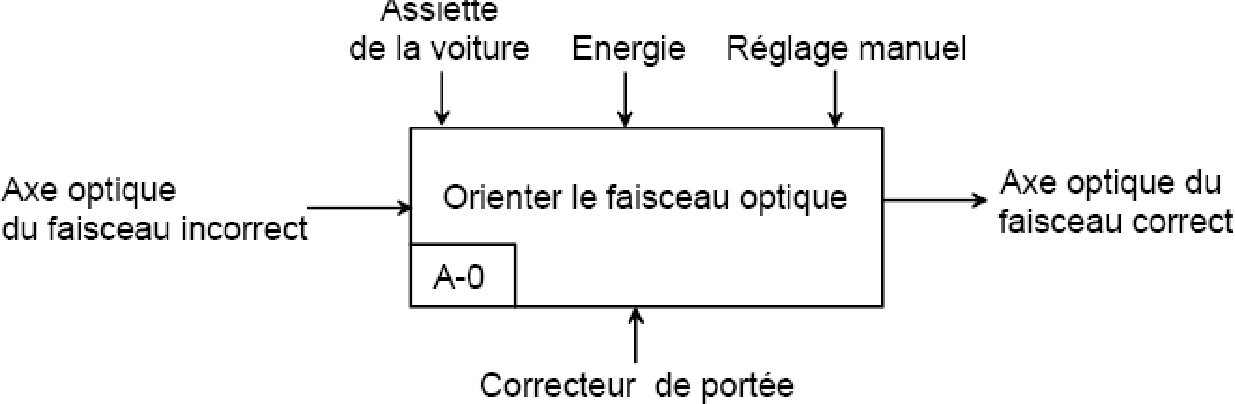
\includegraphics[width=.9\linewidth]{images/image1_3}
\end{center}

\subsection*{Étude de la chaîne d’action complète}
La chaîne d‘action complète comprend :
\begin{itemize}
 \item l‘ensemble transducteur (\textbf{capteur + amplificateur + calculateur})
qui mesure l‘angle de tangage $\beta$ du véhicule et commande le moteur du
système. L‘ensemble est assimilable à un gain pur : $K_c$;
\item le \textbf{moteur à courant continu} dont la fonction de transfert est
notée $M(p)$;
\item on équipe ce moteur d‘un retour tachymétrique assimilable à un gain pur : 
   $K_{tachy}=0,03 V.rad^{-1}.s$;
\item le \textbf{réducteur de vitesse} dont le rapport de réduction est de 490;
\item l’ensemble \textbf{vis-écrou} (de pas $p = 6mm$) qui transforme la
rotation de l’axe du réducteur en translation de l’axe de sortie. (NB : 1
tour de la vis fait avancer de 1 pas l’écrou);
\item le \textbf{bloc d‘orientation} : l‘angle de correction de portée
$\theta(t)$ étant petit, on peut linéariser la loi entrée-sortie sur le
domaine d‘utilisation ; l‘angle $\theta(t)$ est proportionnel au déplacement
$x(t)$ de la vis.
\end{itemize}

($\theta(t)$ varie entre $\dfrac{-\pi}{20}$ $\dfrac{\pi}{20}$ et pour
$x(t)$ compris entre -15mm et +15mm).

\subparagraph{}
\textit{Refaire, sur votre copie, le diagramme fonctionnel de la chaîne d‘action
ci-dessous, en précisant le nom des constituants dans les blocs, les
informations véhiculées entre les blocs ainsi que leur symbole et leur unité
(les fonctions de transfert ne seront pas déterminées).}
NB : 
\begin{itemize}
 \item l’entrée $B(p)$ est la transformée de Laplace de $\beta(t)$ et la sortie
$\Theta(p)$, la transformée de Laplace de $\theta(t)$;
\item attention, un bloc modélise le passage de la vitesse angulaire $\Omega(p)$
à la position angulaire $\Theta(p)$.
\end{itemize}

\begin{center}
 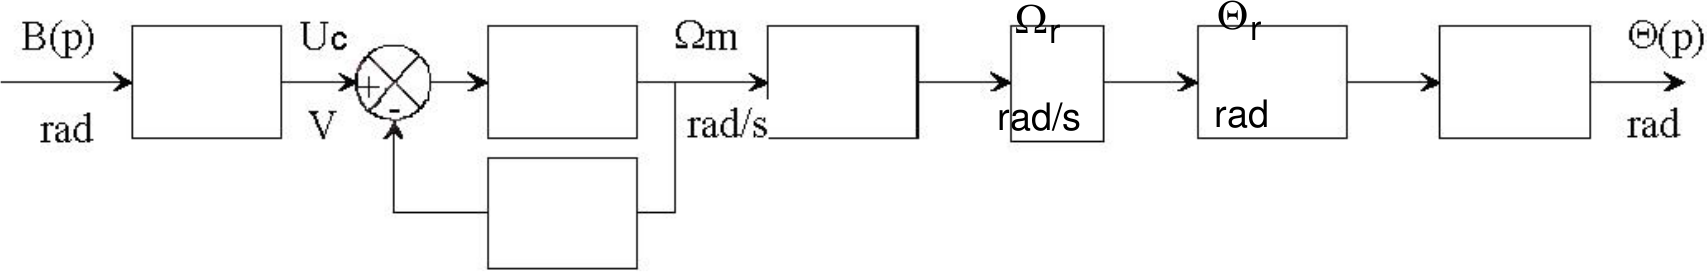
\includegraphics[width=.9\linewidth]{images/image1_4}
\end{center}

\subparagraph{}
\textit{Refaire, sur votre copie, le diagramme fonctionnel de la chaîne d‘action
ci-dessus, mais cette fois-ci en précisant les fonctions de transfert de chaque
bloc.}

Pour déterminer la fonction de transfert du moteur, $M(p)$, on dispose de sa
réponse indicielle (entrée unitaire) :

\begin{center}
 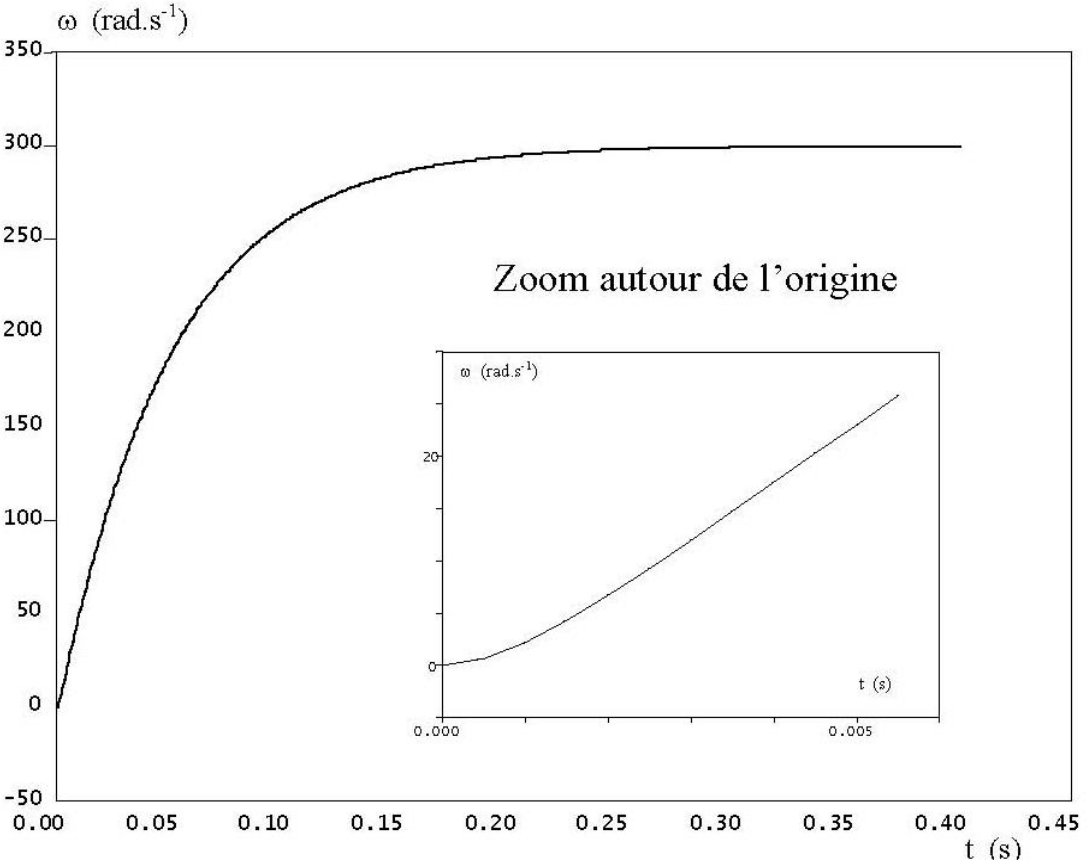
\includegraphics[width=.9\linewidth]{images/image1_5}
\end{center}

\subparagraph{}
\textit{Quelle est la forme de la fonction de transfert du moteur et pourquoi ?}

\subparagraph{}
\textit{Quelle hypothèse pouvons-nous faire pour modéliser le système par un
système du 1\up{er}
ordre ?
NB : Pour démontrer ce raisonnement, déterminer la réponse temporelle d’un
système
du 2\up{ème} ordre apériodique, puis simplifier cette réponse avec votre
hypothèse et enfin
conclure.
Cette hypothèse vous semble-t-elle justifiée ici au vu de la réponse indicielle.
}

\subparagraph{}
\textit{Identifier $M(p)$ à un 1\up{er} ordre. (Pour cela déterminer les
paramètres caractéristiques sur la courbe).}

\subparagraph{}
\textit{En déduire la fonction de transfert $M'(p)=\dfrac{\Omega_m(p)}{U_c(p)}$
du moteur équipé du retour                                                 
tachymétrique. Quels sont les avantages et les inconvénients de cette boucle de
retour ?}

La fonction de transfert de la chaîne d‘action complète est donnée
approximativement par :
$H(p)=\dfrac{\Theta(p)}{B(p)}=K_c\dfrac{0,003}{\left(1+0,025p \right)p}$    
(Les angles d‘entrée et de sortie sont exprimés en radian).

Le véhicule est brusquement chargé à l‘arrière.

\subparagraph{}
\textit{Tracer, SANS FAIRE DE CALCUL, l‘allure de la loi d‘entrée, puis l‘allure
de la réponse.
Justifier votre tracé. Est-ce satisfaisant ?
}

Pour remédier à ce problème on asservit le système en position en plaçant :
\begin{itemize}
 \item un capteur de position, de gain $K_{pos}$ , qui mesure l‘angle $\theta$,
\item un amplificateur de gain pur $A$.
\end{itemize}

\begin{center}
 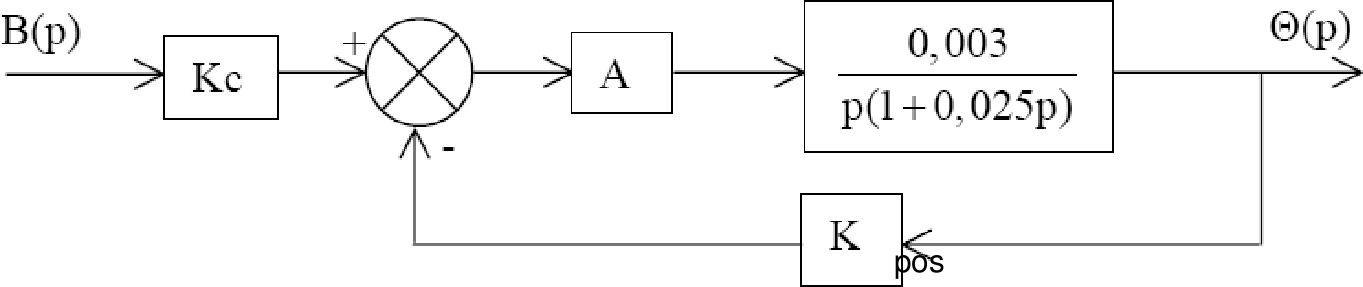
\includegraphics[width=.9\linewidth]{images/image1_6}
\end{center}

\subparagraph{}
\textit{Déterminer la nouvelle fonction de transfert $\dfrac{\Theta(p)}{B(p)}$
ainsi que ses paramètres caractéristiques.
}

\subparagraph{}
\textit{Expliquer en deux lignes pourquoi le problème a été remédié.}

\subparagraph{}
\textit{À partir de la courbe ci-contre, déterminer la quantité $AK_{pos}$ qui
permet d‘avoir le système le plus rapide. Calculer alors le temps de réponse à
5\% du système.}

\begin{center}
 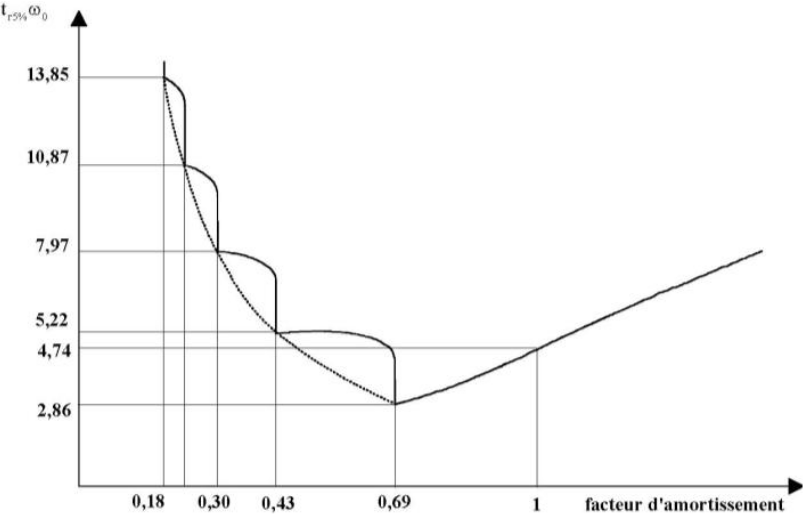
\includegraphics[width=\linewidth]{images/image1_7}
\end{center}

\newpage
\setcounter{exo}{0}
\section*{Étude du plan horizontal réglable (PHR) de l'airbus A340}


\begin{flushright}
\textit{D'après ressources d'Alain Caignot.}
\end{flushright}
\subsection*{Présentation}
Le thème proposé concerne l'aéronautique et plus particulièrement la commande en position du plan horizontal réglable (PHR) de l'airbus A340. 

%Gros porteur, très long courrier, ce quadriréacteur symbolise l'aboutissement de la politique de la gamme menée par le conducteur européen depuis le commercialisation de son premier avion, l'A300.
%
%\begin{center}
%\begin{tabular}{ccc}
%\hline
%Spécifications & A340-500 & A340-600 \\
%\hline
%\hline
%Longueur & 67,90 m & 75,30 m \\
%Envergure & 63,45 m & 63,45 m  \\
%Surface ailaire & 437 $m^2$ & 437 $m^2$  \\
%Capacité en sièges & 313 & 378 \\
%Autonomie (km)/Nm & 15.800/8.500 & 13.900/7.500 \\
%Poids au décollage & 368 t & 369 t \\
%Capacité des réservoirs & 214.800 & 194.880 \\
%Moteurs & Trent 553 & Trent 556 \\
%Puissance des moteurs (lbs) & 53.000 & 56.000 \\
%\hline
%\end{tabular}
%\end{center}
%
%\begin{center}
%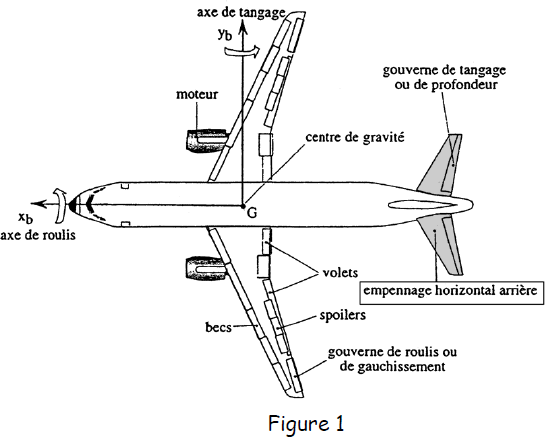
\includegraphics[width=.65\textwidth]{images/image2_2}
%\end{center}
%
%Le PHR est réglé à l’aide des gouvernes de profondeur (voir Figure 1). On peut montrer que pour une
%vitesse donnée, il est possible, par réglage du PHR, de réduire la poussée des réacteurs et donc
%d’économiser du carburant.
%
%Afin de répondre aux exigences de fiabilité qui stipulent, en particulier, que le PHR doit pouvoir
%fonctionner durant 109 FH (Fly Hour) sans subir de défaillance, un certain nombre de composants de la
%chaîne de commande du PHR sont doublés ou triplés suivant les cas.
%
%D’autre part, toujours par souci de sécurité, le PHR peut être commandé :
%\begin{itemize}
%\item soit automatiquement par un ordinateur de bord qui détermine, à partir des paramètres du vol,
%la valeur optimale de l’angle $\beta$ que doit prendre les gouvernes de profondeur,
%\item soit manuellement par le pilote à partir d’un volant de commande situé dans le poste de pilotage
%et ce en cas de défaillance de la commande automatique du PHR.
%\end{itemize}
%
%La figure 2 présente le schéma de principe de la chaîne d’action à partir de la génération de la
%commande par le calculateur ou le pilote.

Le calculateur génère une tension de commande qui va alimenter le moteur électrique qui est asservi en
position angulaire pour permettre de générer l’angle de consigne initial. Cet angle de consigne initial est
adapté à l’aide du réducteur 1. L’angle de sortie du réducteur 1 permet de commander les deux
distributeurs proportionnels, qui vont délivrer un débit de fluide hydraulique pour alimenter les deux
moteurs hydrauliques. Ces deux moteurs hydrauliques transforment l’énergie hydraulique en énergie
mécanique de rotation. Les deux mouvements de rotation ainsi générer sont additionnés à l’aide du
différentiel pour créer un seul mouvement de rotation à sa sortie. La sortie du différentiel est reliée
au réducteur 6 qui va adapter l’énergie mécanique de puissance pour actionner la vis 4. La vis 4 est
reliée à la gouverne de profondeur et permet de commander son angle.

L’angle de rotation de la vis 4 est capté à l’aide du réducteur 7 qui va l’adapter afin d’être comparé à la
rotation de commande des distributeurs à l’aide du train épicycloïdal, qui joue ici le rôle d’un
comparateur.


%
%\subsection*{Analyse fonctionnelle}
%\subparagraph{Question 1}
%\textit{Compléter le diagramme FAST relatif à la fonction principale régler l’angle du PHR sur le
%document réponse DR1.}
%
%
%\begin{center}
%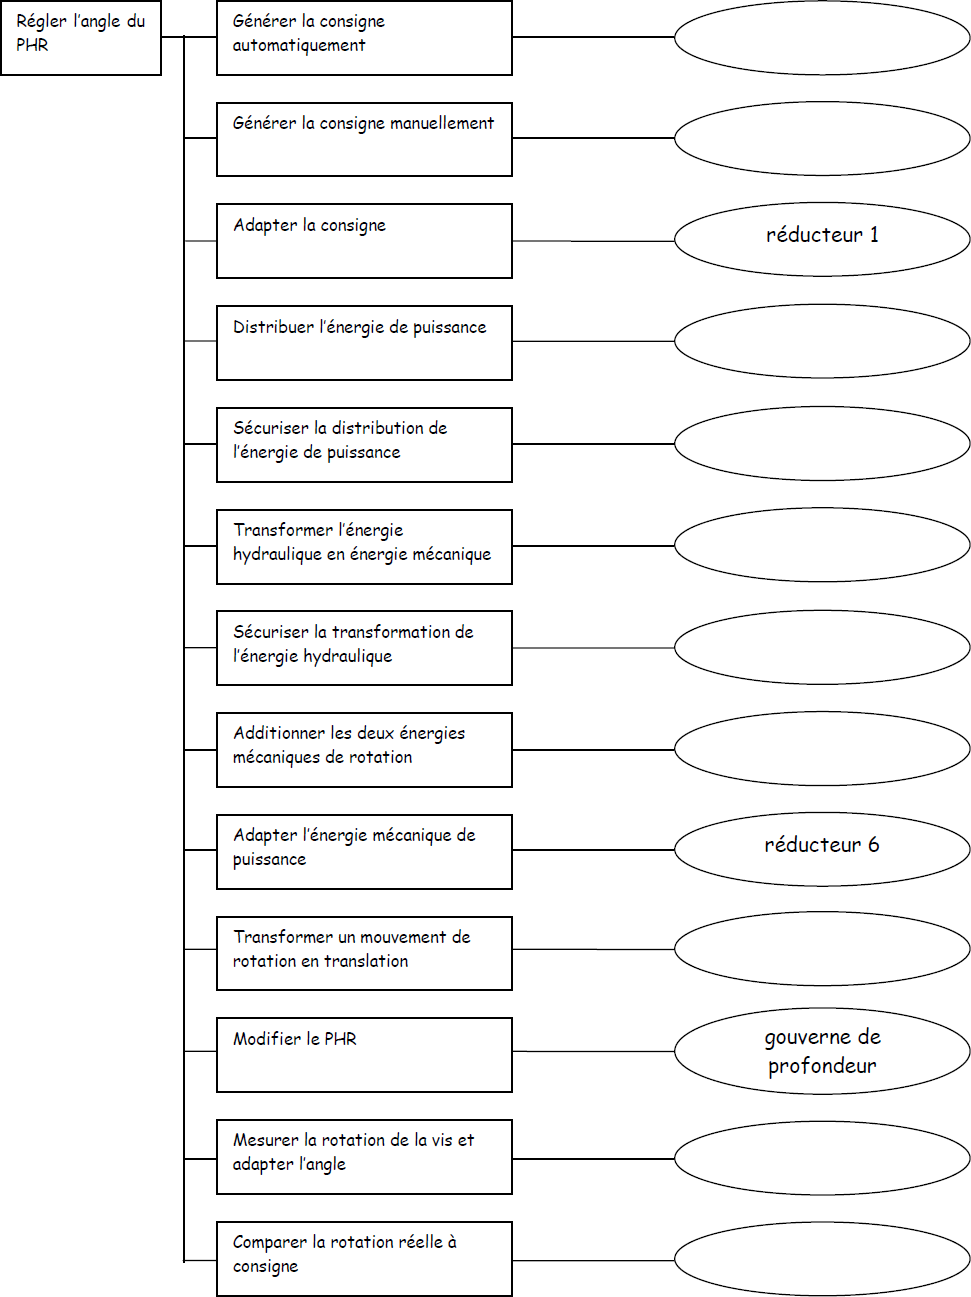
\includegraphics[width=\textwidth]{images/image2_6}
%\end{center}

\begin{center}
%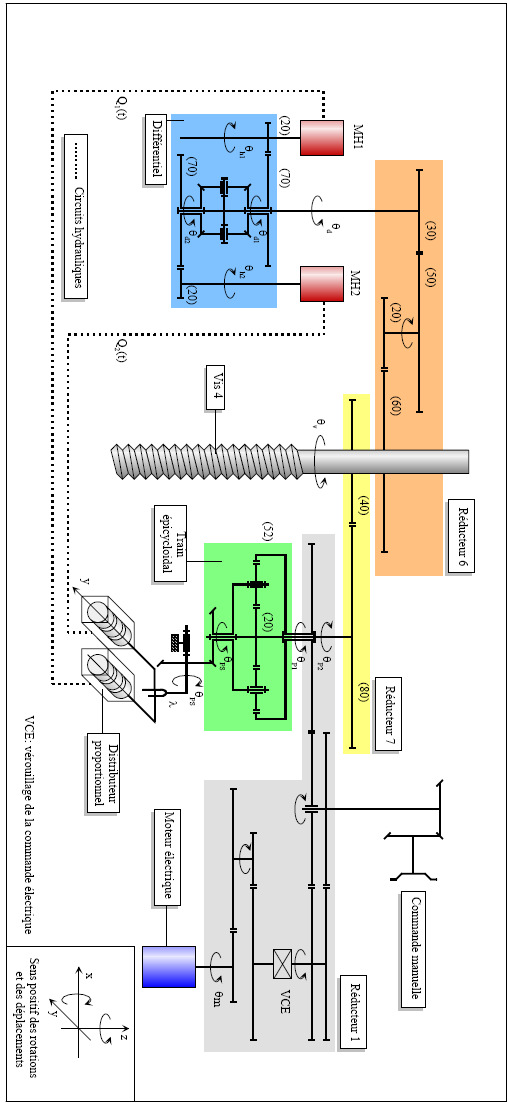
\includegraphics[height=.95\textheight]{images/image2_3}
\rotatebox{90}{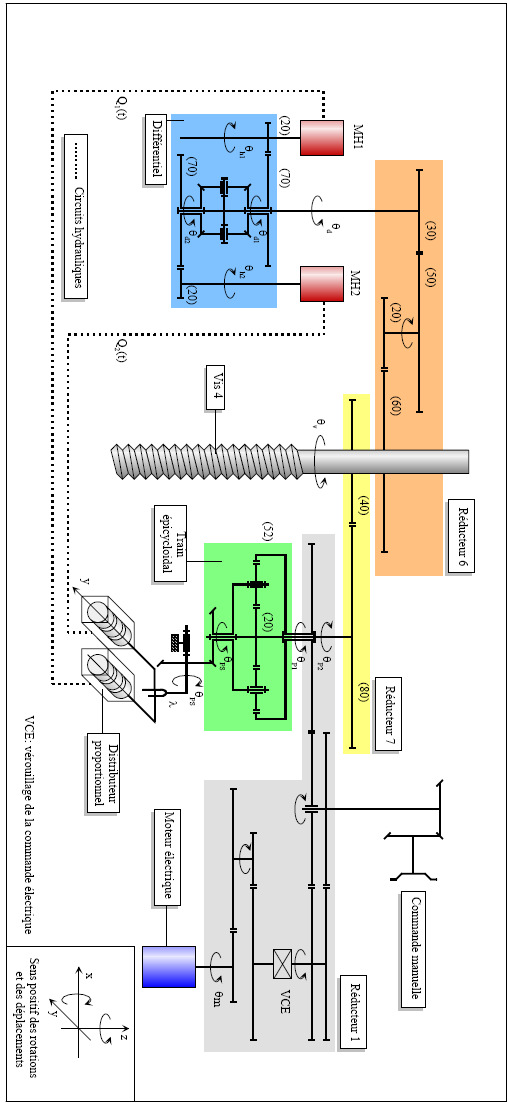
\includegraphics[height=\linewidth]{images/image2_3}}

Figure 3
\end{center}

\subsection*{\'Etude de l'asservissement en position du moteur électrique}
%
%On se propose d'étudier précisément la boucle d'asservissement en position angulaire du moteur électrique. L'entrée de cet asservissement est une tension de consigne $U_e$ générée par le calculateur. Cette tension est comparée à une tension $U_r$, image de l'angle $\theta_r$, délivrée par un capteur potentiométrique. L'écart $\varepsilon_1$ est ensuite corrigé et amplifié par un bloc correcteur et amplificateur et fournit la tension $U$ aux bornes du moteur électrique. L'angle de rotation $\theta_m$ en sortie du moteur est réduit par un réducteur \textbf{2} pour donner la rotation $\theta_r$ mesurée par le capteur. D'autre part, l'angle $\theta_m$ est réduit par un réducteur \textbf{1} pour fournir un angle de rotation en sortie $\theta_{P1}$, sortie de cet asservissement. 
%
%\subparagraph{Question 2}
%\textit{Construire le schéma bloc fonctionnel de cet asservissement.}

\subsection*{Analyse du moteur électrique}
Le moteur électrique est un moteur à courant continu. Les ingénieurs procèdent à une identification du
moteur en le soumettant à un échelon de tension $U=5V$, afin de déterminer par un modèle de
comportement sa fonction de transfert. On obtient la réponse indicielle (vitesse de rotation $\omega_m(t)$ )
donnée ci-après.

\subparagraph{}
\textit{Identifier la réponse en justifiant le modèle retenu et la (ou les) techniques utilisées pour
déterminer les paramètres. Les tracés seront laissés apparents sur la figure ci-après.}


\begin{center}
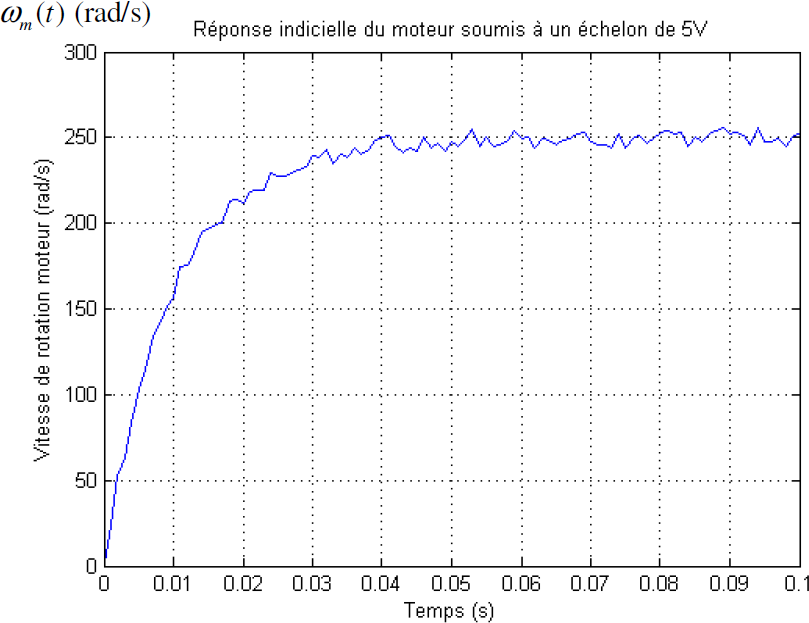
\includegraphics[width=\linewidth]{images/image2_7}
\end{center}


Pour valider le modèle expérimental, on peut utiliser les équations du moteur à courant continu :
\begin{itemize}
\item équation électrique liant la tension $u$ aux bornes du moteur et le courant $i$ le traversant :
$u(t) = Ri(t) + e(t)$;
\item équation de couplage électrique liant la tension contre-électromotrice $e(t)$ à la vitesse de
rotation $\omega_m(t)$ de l’arbre du moteur et le couple moteur : $e(t)= k_e \omega_m(t)$;
\item équation de la mécanique liant la vitesse de rotation $\omega_m(t)$  et le couple moteur $C_m(t)$ :
$J_e \dfrac{d\omega_m(t)}{dt} = C_m(t)$;
\item équation de couplage mécanique liant le couple moteur au courant : $C_m(t)=k_ai(t)$
\end{itemize}

Avec :
\begin{itemize}
\item $R$ : la résistance de l'induit  ($R=1\Omega$);
\item $J_e$ : inertie équivalente ramenée sur l’arbre moteur ($J_e=4\cdot10^{-6} \;  kg\cdot m^2$);
\item $k_e$ : constante de force contre électromotrice ($k_e=0,02V/(rad/s)$);
\item $k_a$ : constante de couple ($k_a=0,02 Nm/A$).
\end{itemize}

\subsection*{Détermination de la fonction de transfert du moteur}
\subparagraph{}
\textit{Déterminer la fonction de transfert $M(p)=\dfrac{\theta_m(p)}{U(p)}$ du moteur électrique et montrer qu'elle peut se mettre sous la forme d'un intégrateur $1/p$ multiplié par une fonction de transfert d'un 1\up{er} ordre de gain statique $K_m$ et de constante de temps $\tau_m$.}

\subparagraph{}
\textit{Donner les expressions littérales de $K_m$ et $\tau_m$.}

\subparagraph{}
\textit{Application numérique : calculer $K_m$ et $\tau_m$ en précisant les unités.}


\subsection*{Schéma bloc de l'asservissement}
La fonction de transfert du correcteur et amplificateur peut être assimilé dans un gain $K_1$. La fonction de transfert du réducteur \textbf{2} est un gain noté $R_2$. La fonction de transfert du réducteur \textbf{1} est un gain noté $R_1$. La fonction de transfert du capteur potentiométrique est assimilée à un gain noté $K_2$.

%\subparagraph{}
%\textit{Montrer que le schéma-bloc peut se mettre sous la forme suivante :}
 Les schéma bloc peut se mettre sous la forme suivante :
\begin{center}
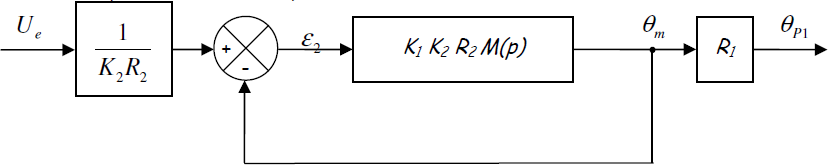
\includegraphics[width=\linewidth]{images/image2_4}
\end{center}

Le rapport de transmission du réducteur \textbf{1} est $R_1=\dfrac{1}{150}$.

\subsection*{Détermination de la fonction de transfert en boucle ouverte}
\subparagraph{}
\textit{Déterminer la fonction de transfert $T(p)=\dfrac{\theta_{m}(p)}{\varepsilon_2(p)}$, la mettre sous la forme 
$T(p)=\dfrac{K_{BO}}{p\left( 1+\tau_m p\right)}$ et en déduire l'expression du gain de la boucle $K_{BO}$.}

\subsection*{Détermination de la fonction de transfert en boucle fermée}
\subparagraph{}
\textit{Déterminer la fonction de transfert $F(p)=\dfrac{\theta_{P1}(p)}{U_e(p)}$ et montrer qu'elle peut se mettre sous la forme d'un système du second ordre. On notera $K_{BF}$ le gain statique $\xi$ le coefficient d'amortissement et $\omega_0$ la pulsation propre.}

\subparagraph{}
\textit{Donner l'expression littérale de $K_{BF}$ en fonction de $R_1$, $R_2$ et $K_2$ de $\xi$ et $\omega_0$ en fonction de $K_{BO}$ et $\tau_m$.}


\subsection*{Analyse des performances}
\subparagraph{\label{ques}}
\textit{Déterminer la valeur du gain de boucle $K_{BO}$ de telle sorte que la réponse à une entrée de type échelon soit la plus rapide possible sans toutefois produire de dépassement.}

\subparagraph{}
\textit{Déterminer l'écart de position pour une entrée de type échelon en calculant l'écart statique : 
$\varepsilon_s = \lim\limits_{t\to +\infty}\varepsilon_2(t)$. Le système est précis à une entrée de type échelon si $\varepsilon_S=0$. Conclure.}

\subparagraph{}
\textit{Déterminer le temps de réponse à 5\% à l'aide de la figure 3.}


\begin{center}
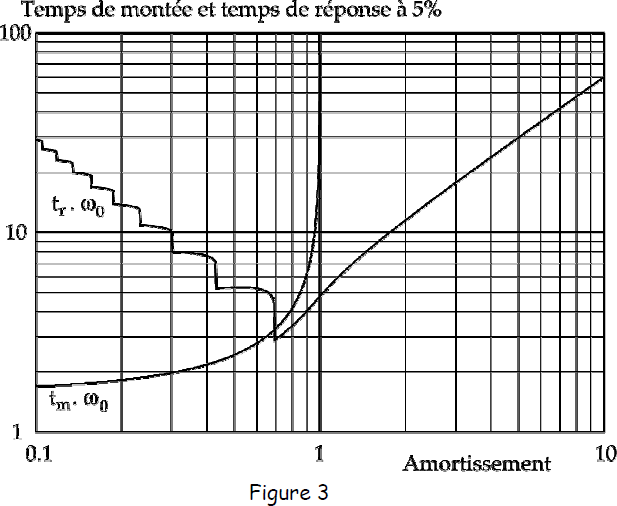
\includegraphics[width=\linewidth]{images/image2_5}
\end{center}



%\subsection{Détermination du gain $K_1$}
%On admet que la longueur utile de la vis est $l = 0,6\;m$. Le pas de la vis est $p_v=10\;mm$ (distance
%parcourue quand la vis à fait un tour).
%
%\subparagraph{}
%\textit{Déterminer le nombre de tour maximal $N_v$ que va faire la vis.}
%
%La vis est entraînée en rotation par un réducteur \textbf{52} dont le rapport de réduction est 
%$\dfrac{\theta_{P1}}{\theta_v}=\dfrac{1}{5}$.
%
%
%\subparagraph{}
%\textit{Déterminer le nombre de tour $N_{P1}$ que va faire l’arbre d’entrée du réducteur \textbf{52}.
%L’arbre d’entrée du réducteur \textbf{52} est entraîné par le réducteur \textbf{1}.}
%
%\subparagraph{}
%\textit{En déduire le nombre de tour $N_m$ que va faire l’arbre du moteur.}
%
%Le capteur de position de gain $K_2$ de la boucle d’asservissement du moteur électrique est un capteur
%potentiométrique 10 tours dont la tension de sortie varie de -12 à +12 Volts.
%
%\subparagraph{}
%\textit{En supposant que l’on utilise le capteur sur toute sa plage (10 tours), déterminer le rapport
%de réduction $R_2$ du réducteur reliant la sortie du moteur à l’entrée du potentiomètre.}
%
%\subparagraph{}
%\textit{Déterminer le gain du capteur potentiométrique.}
%
%\subparagraph{}
%\textit{En déduire le gain $K_1$ du régulateur connaissant la valeur de $K_{BO}$ fixée lors de la \textbf{Question \ref{ques}}.}

\subsection*{Analyse des performances en mode suiveur}
Dans le cas d’une entrée de type rampe $u_e(t) = t u(t)$, le cahier des charges stipule que l’écart de
traînage ne doit pas excéder $\varepsilon_T \leq 0,5\;rad$.

\subparagraph{}
\textit{Déterminer l’écart de traînage $\varepsilon_T =\lim\limits_{t\to +\infty} \varepsilon_2(t)$ à une entrée de type rampe.}

\subparagraph{}
\textit{En déduire une première inégalité sur $K_{BO}$ permettant de vérifier cette partie du cahier
charges.}

\subparagraph{}
\textit{En reprenant la \textbf{Question \ref{ques}}, déterminer une seconde inégalité sur $K_{BO}$ permettant d’assurer que la réponse indicielle du système ne présentera pas de dépassement.}

Dans la pratique le régulateur est un correcteur dont la fonction de transfert est :
$$
C_1(p)=K_1\dfrac{1+T_1 p}{1+bT_1 p} \text{ avec } b>1
$$


\subparagraph{}
\textit{Justifier la nécessité de ce correcteur.}

\newpage

\section*{Robot préhenseur}
\setcounter{exo}{0}

\begin{flushright}
\textit{D'après ressources Florestan Mathurin.}
\end{flushright}



Le support de l'étude est un préhenseur de pièces. Il permet à l'utilisateur de prendre des pièces pour les déplacer. L'application illustrée sur l'image ci-dessous est la prise de bouteilles plastiques sur un tapis roulant, afin de les trier pour faire du recyclage. 

\vspace{0.25cm}

\begin{center}
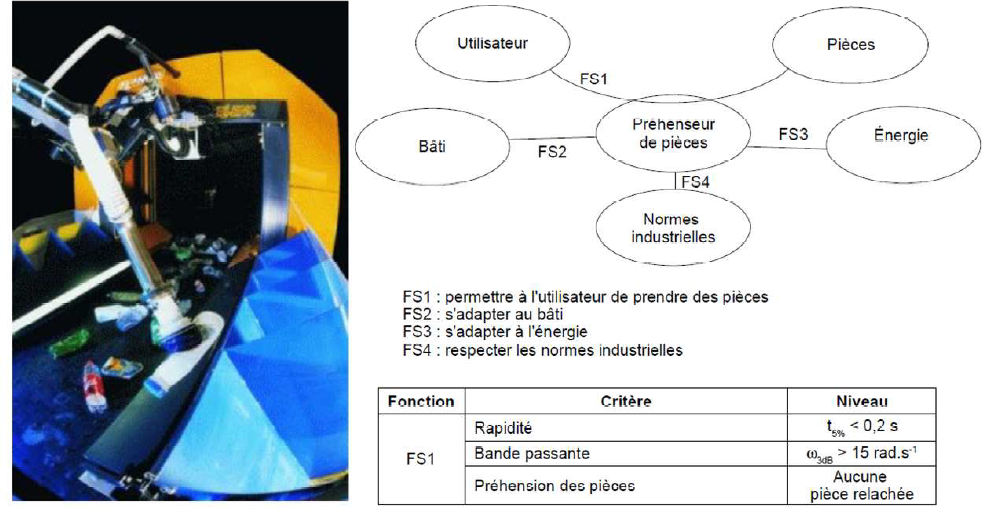
\includegraphics[width=\linewidth]{images/fig2}
\end{center}
%\begin{minipage}[c]{.3\linewidth}
%\begin{center}
%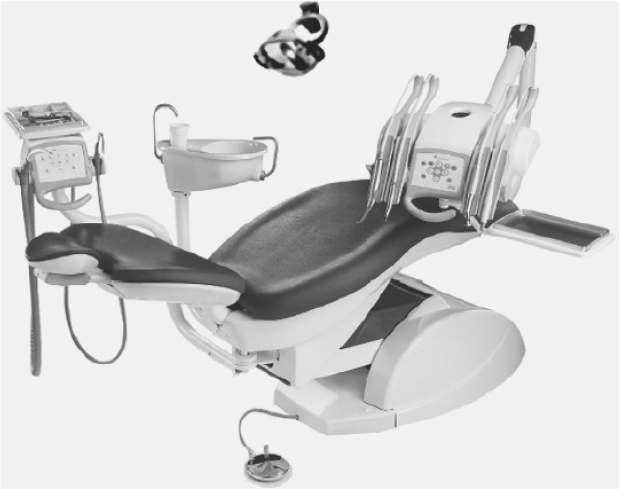
\includegraphics[width=.9\textwidth]{images/fig1}
%\end{center}
%\end{minipage}\hfill
%\begin{minipage}[c]{.65\linewidth}
%\begin{center}
%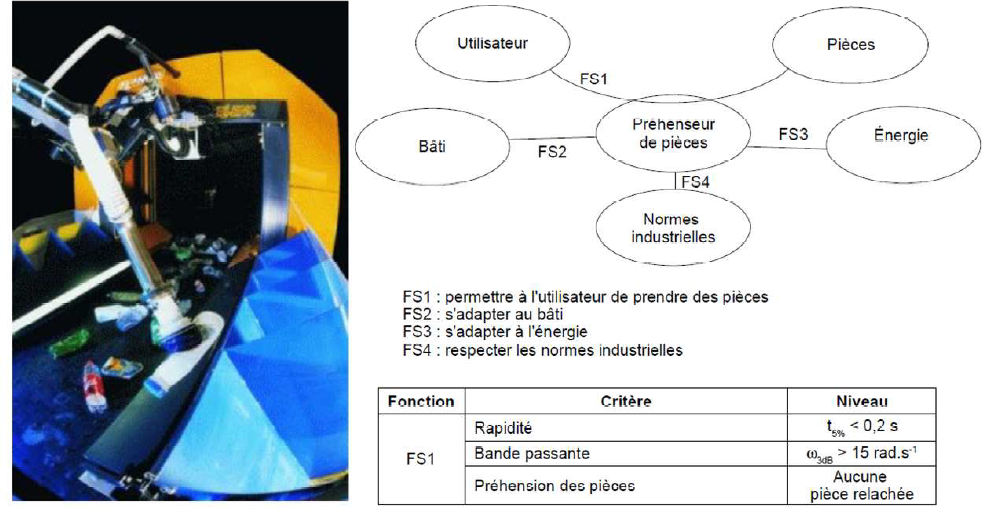
\includegraphics[width=.9\textwidth]{images/fig2}
%\end{center}
%\end{minipage}

L'objectif de cette étude est de vérifier les performances de la fonction FS1, décrites dans le cahier des charges de ce système. On réalise l'asservissement de la position angulaire d'un bras du préhenseur de pièces, selon le schéma bloc qui suit (l'angle du bras $\theta_b(t)$, l'angle consigne est $\theta_c(t)$).

\begin{center}
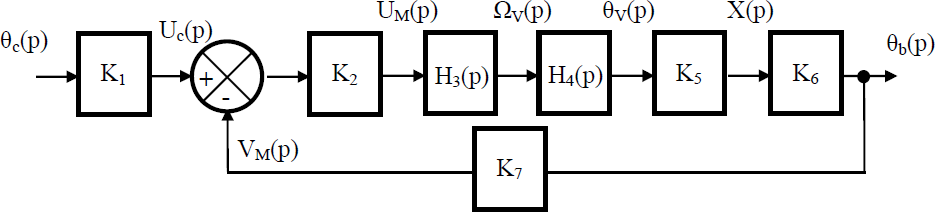
\includegraphics[width=\linewidth]{images/fig_3}
\end{center}

Avec $K_1$, $K_2$, $K_5$, $K_6$ et $K_7$ : constantes, $\theta_c(p)$ : angle de consigne, $U_c(p)$ : tension de consigne, $U_M(p)$, tension moteur, $\Omega_V(p)$ : vitesse angulaire de la vis, $\theta_V(p)$ : angle de la vis, $X(p)$ : déplacement de l'écrou, $\dot{\theta_b(p)}$ : position angulaire du bras, $V_M(p)$ : tension mesurée image de $\theta_b(p)$.

\subparagraph{}
\textit{Déterminer le lien entre $K_1$ et $K_7$ pour que $\theta_b(p)$ soit asservi sur $\theta_c(p)$.}

La fonction de transfert $H_3(p)$ est réalisée par un moteur, dont les équations de comportement sont :
$u_M(t)=e(t)+R\cdot i(t)$, $e(t)=k_e\omega_v(t)$, $J\cdot \dfrac{d\omega_v(t)}{dt}=C_M(t)$, $C_M(t)=k_M i(t)$.


Avec $u_M(t)$ : tension aux bornes du moteur (en V), $e(t)$ : force contre-électromotrice (en V), $i(t)$ intensité (en A), $\omega_V(t)$ : vitesse de rotation de la vis en sortie de moteur (en rad/s), $C_M(t)$ ; couple moteur (en N.m) (un couple est une action mécanique qui tend à faire tourner). $J$ inertie équivalente en rotation de l'arbre moteur (en $kg\cdot m^2$), $R$ résistance du moteur (en $\Omega$), $k_e$ constante de force contre-électrmotrice ($V\cdot rad^{-1}\cdot s$), $k_m$ : constante de couple ($N\cdot m\cdot A^{-1}$).

\subparagraph{}
\textit{Déterminer la fonction de transfert $H_3(p)=\dfrac{\Omega_V(p)}{U_M(p)}$. Montrer que $H_3(p)$ peut se mettre sous la forme canonique d'un système du premier ordre où les valeurs $K_3$ et $T_3$ seront à déterminer.}

\subparagraph{}
\textit{Déterminer $\omega_v(t)$ lorsque $u_M(t)$ est un échelon de tension d'amplitude $U_0$. Préciser la valeur de $\omega_v(t)$ à l'origine, la pente de la tangente à l'origine de $\omega_V(t)$ et la valeur finale atteinte par $\omega_V(t)$ lorsque $t$ tend vers l'infini.}

\subparagraph{}
\textit{Déterminer la fonction de transfert $H_4(p)$. }

\subparagraph{}
\textit{Déterminer la fonction de transfert $H(p)=\dfrac{\theta_b(p)}{\theta_c(p)}$. Montrer que cette fonction peut se mettre sous la forme d'un système du second ordre ou les valeurs de $K$, $z$ et $\omega_0$ seront à déterminer.}

La réponse indicielle de $H(p)$ à un échelon unitaire est donnée sur la figure suivante :

\begin{center}
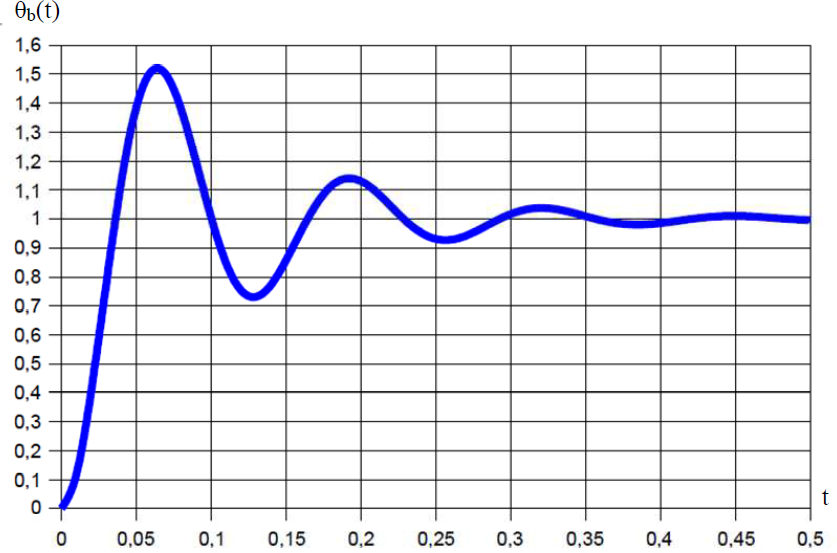
\includegraphics[width=\linewidth]{images/fig_4}
\end{center}

\subparagraph{}
\textit{Déterminer, en expliquant la méthode, les valeurs numériques de $K$, $z$ et $\omega_0$.}

\subparagraph{}
\textit{Déterminer, en expliquant la démarche utilisée, le temps de réponse à 5\%. Conclure quant à la capacité du préhenseur à vérifier (ou non) le critère de rapidité de FS1.}


\newpage
\setcounter{exo}{0}


%\begin{flushright}
%\textit{D'après ressources d'Alain Caignot.}
%\end{flushright}




\section*{Unité dentaire}
\textit{(Selon le concours E3A PSI 2007)}
\setcounter{exo}{0}


Le support de l'étude est une "unité dentaire" dont on donne un extrait du cahier des charges fonctionnel. Cet équipement a été conçu et réalisé dans le but d'une adaptabilité maximale aux différentes méthodes de travail des chirurgiens dentistes. Son ergonomie, sa maniabilité, son design, sa fiabilité en font une "unité universelle". Sa conception est modulaire avec une technologie avancée.

Le chirurgien dentiste possède une pédale et un pupitre de commande, qui lui permet de monter ou descendre verticalement le corps du patient, de l'incliner plus ou moins, et de positionner sa tête. Le patient pouvant prendre une position spatiale pertinente, tous les actes médicaux sont facilités.

\begin{center}
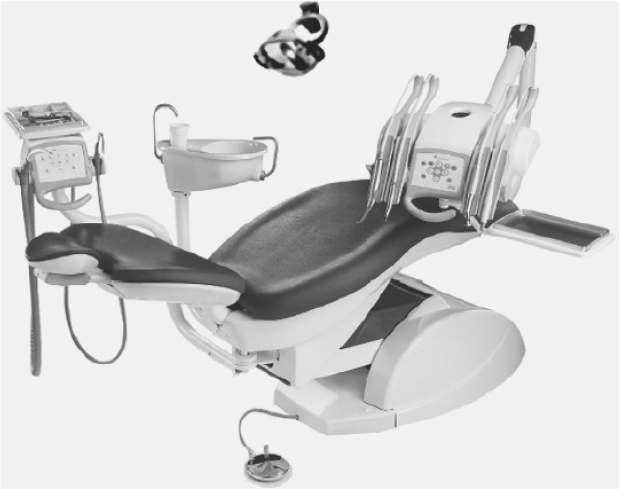
\includegraphics[width=\linewidth]{images/fig1}
\end{center}


\begin{center}
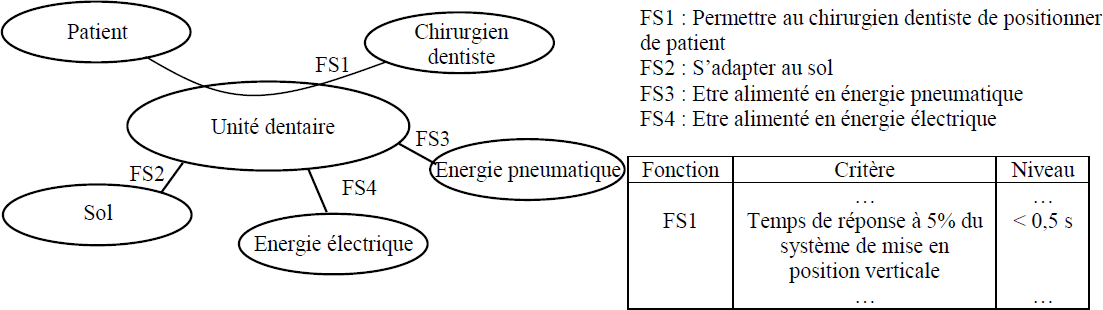
\includegraphics[width=.9\linewidth]{images/fig4_2}
\end{center}

On s'intéresse dans ce sujet au critère de la FS1 concernant le temps de réponse du système permettant de mettre en position verticale le patient. 

Pour régler le patient en position verticale, le chirurgien dentiste appuie sur une pédale, plus ou moins fort. Un moteur électrique se met en route, sa vitesse de rotation dépend de l'appui plus ou moins profond du chirurgien dentiste sur la pédale. La vitesse de rotation du moteur est diminuée par un réducteur à engrenages. En sortie du réducteur à engrenages se trouve une vis dont la rotation $\Omega_v(p)$ entraîne, par un système vis-écrou, la translation du siège en hauteur. L'ensemble peut se représenter par le schéma bloc suivant. Le composant de fonction de transfert $C(p)$ est un correcteur :


\begin{center}
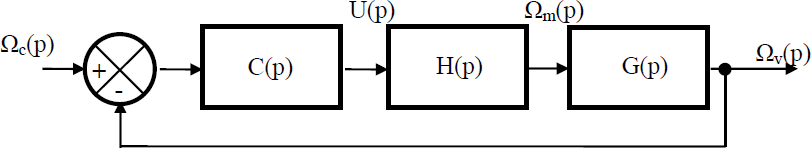
\includegraphics[width=\linewidth]{images/fig3}
\end{center}

\subparagraph{}
\textit{Déterminer le nom des composants qui réalisent les fonctions $H(p)$ et $G(p)$.}

\subparagraph{}
\textit{Déterminer la fonction de transfert en boucle fermée du système $\dfrac{\Omega_v(p)}{\Omega_c(p)}$.}

Les équations du moteur utilisé sont les suivantes : $u(t)=e(t)+Ri(t)+L\dfrac{di(t)}{dt}$, $e(t) = k_e \omega_m(t)$, $ J\cdot\dfrac{d\omega_m(t)}{dt} = C_m(t)-f\omega_m(t)$, $ C_m(t)=k_m \cdot i(t)
$

On note $u(t)$ tension du moteur, $e(t)$, la force contre électro motrice du moteur, $i(t)$ l'intensité dans le moteur, $C_m(t)$ le couple exercé par le moteur et $\omega_m(t)$ la vitesse angulaire du moteur. Les grandeurs physiques $R$, $L$, $k_e$, $J$, $f$ et $k_m$ sont des constantes.

\subparagraph{}
\textit{En supposant les conditions initiales nulles, exprimer ces équations dans le domaine de Laplace.}

\subparagraph{}
\textit{Montrer que, dans le domaine de Laplace, la relation entre $\Omega_m(p)$ et $U(p)$ peut s'écrire sous la forme d'une fonction de transfert du second ordre. On déterminera les différentes constantes.}

Si on utilise un correcteur proportionnel, l'application numérique des grandeurs physiques permet de trouver la fonction suivante : $\dfrac{\Omega_v(p)}{\Omega_c(p)} =\dfrac{K_T}{1+T_T p}$ avec $K_T=0,9$ et $T_T=0,1 s.$.

\subparagraph{}
\textit{Déterminer $\omega_v(t)$ lorsque le chirurgien dentiste demande un échelon de rotation $\omega_c(t)=\omega_{c0}\cdot u(t)$. Exprimer le résultat en fonction de $\omega_{C0}$, $K_T$ et $T_T$.}

\subparagraph{}
\textit{Déterminer le temps de réponse à 5\% du système et effectuer l'application numérique. Conclure vis-à-vis du cahier des charges.}

Le patient, initialement immobile, bouge verticalement selon le déplacement $x_v(t)$ tel que $\dfrac{dx_v(t)}{dt} = a\omega_v(t)$ avec $a$ constante qui représente le pas réduit de la vis. 

\subparagraph{}
\textit{Déterminer la transformée de Laplace $X_v(p)$ de $x_v(t)$.}

\subparagraph{}
\textit{Déterminer $x_v(t)$ en fonction de $a$, $K_T$, $T_T$ et $\omega_{c0}$.}


Si on utilise un correcteur proportionnel, dérivé et intégral, l'application numérique des grandeurs physiques permet de trouver la fonction suivante : $\dfrac{\Omega_v(p)}{\Omega_c(p)} = \dfrac{1}{1+2p+p^2}
$

\subparagraph{}
\textit{Déterminer $\omega_v(t)$ lorsque le chirurgien dentiste demande un échelon de rotation $\omega_c(t)=\omega_{c0}\cdot u(t)$.}

\subparagraph{}
\textit{Déterminer si le temps de réponse à 5\% est plus faible  ou plus grand que dans le cas précédent. Conclure vis-à-vis du cahier des charges.}

\end{multicols}



\end{document}


